\documentclass[10pt]{article}
\usepackage[left=0.9in,top=0.9in,bottom=0.9in,right=0.9in]{geometry}
\usepackage{setspace}
\usepackage{titlesec}
\usepackage{graphicx}
\usepackage{float}
\usepackage{mathtools}
\usepackage{amsmath}
\usepackage[font=small,labelfont=bf,labelsep=period]{caption}
\usepackage[english]{babel}
\usepackage{indentfirst}
\usepackage{array}
\usepackage{makecell}
\usepackage[usenames,dvipsnames]{xcolor}
\usepackage{multirow}
\usepackage{tabularx}
\usepackage{arydshln}
\usepackage{caption}
\usepackage{subcaption}
\usepackage{xfrac}
\usepackage[numbers,sort&compress]{natbib}
\usepackage{enumitem}
\usepackage{lipsum}
\usepackage{hyperref}
\usepackage{caption}
\usepackage{amssymb}
\setlength{\bibsep}{0pt}

\usepackage{listings}
\lstset{
  language=Python,
  aboveskip=3mm,
  belowskip=3mm,
  showstringspaces=false,
  columns=flexible,
  basicstyle={\small\ttfamily},
  breaklines=true,
  breakatwhitespace=true,
  tabsize=3,
  numbers=none,
  xleftmargin=0em,
  framexleftmargin=3.5em
}

%\usepackage{setspace}
%\onehalfspacing
\linespread{1.3}  % one-half spacing

%\pagestyle{fancy} 
%\fancyhead[LE,RO]{\today}
%\fancyhead[C]{NE 255}
%\fancyhead[LO,RE]{D. Hellfeld}
%\fancyfoot[C]{\thepage\ of \pageref{LastPage}}
%\renewcommand{\headrulewidth}{0.4pt}
%\renewcommand{\footrulewidth}{0.4pt}

%\pagestyle{empty}

% Set up figure/table captions
\addto\captionsenglish{\renewcommand{\figurename}{Fig.}}
\addto\captionsenglish{\renewcommand{\tablename}{\small Table}}
\renewcommand{\thetable}{\Roman{table}}
\captionsetup[table]{labelfont = normal, labelsep=period, singlelinecheck=false}
\captionsetup[figure]{labelfont=normal, labelsep=period, singlelinecheck=true}

%\setlength\parindent{0pt}

% Set up section\subsection title formats
\renewcommand{\thesection}{\Roman{section}.}
\renewcommand{\thesubsection}{\small \thesection\Alph{subsection}}
\titleformat*{\section}{\normalsize\bfseries}
\titleformat*{\subsection}{\small\bfseries}

\begin{document}

\begin{centering}
\textbf{Monte Carlo Simulation and Analysis Framework for a CdZnTe-based Spherical Coded\\[-5pt] Aperture and Compton Gamma-ray Imager}\\
\vspace{5pt}
\emph{Final Report}\\
\vspace{5pt}
NE 255 - Numerical Simulation in Radiation Transport \\[-5pt]
University of California, Berkeley \\[-5pt]
Department of Nuclear Engineering\\
\vspace{5pt}
Daniel Hellfeld\\
\vspace{5pt}
December 14, 2016 \\
\end{centering}


% -----------------------------------------------------------------------
\section{Introduction}

Gamma-ray imaging allows for efficient detection, characterization, and localization of compact radioactive sources in complex environments. Fieldable detector systems employing active planar coded masks have demonstrated broad energy sensitivity via both coded aperture (tens to hundreds of keV) and Compton imaging (hundreds of keV to a few MeV) modalities \cite{Galloway2011}. However, the planar configuration of such systems suffer from an inherent limited field-of-view, especially in the case of coded aperture. Lawrence Berkeley National Laboratory (LBNL) has proposed a novel design by rearranging the detectors into an active coded spherical configuration. The Portable Radiation Imaging Spectroscopy and Mapping (PRISM) detector system currently under development (see \hyperlink{fig1}{Fig.\,1a-b}) consists of cm$^3$ CdZnTe (CZT) coplanar grid (CPG) \cite{Luke1995} gamma-ray detectors arranged on the inner surface of a 14 cm diameter spherical housing. There exists 192 available detector locations on the sphere, and an active coded arrangement, or a pattern of occupied and empty locations (see \hyperlink{fig1}{Fig.\,1c}), of the detectors facilitates gamma-ray imaging in 4$\pi$ using both coded aperture and Compton imaging modalities.

% thereby facilitating an isotropic 4$\pi$ field-of-view with both coded aperture and Compton imaging modalities. 

% the Portable Radiation Imaging Spectroscopy and Mapping (PRISM) detector system under development at Lawrence Berkeley National Laboratory (LBNL) (see \hyperlink{fig1}{Fig.\,1a-b}) and to develop a small suite of analysis tools. The PRISM system consists of cm$^3$ CdZnTe (CZT) coplanar grid (CPG) \cite{Luke1995} gamma-ray detectors arranged on the inner surface of a 14 cm diameter spherical housing. There exists 192 available detector locations on the sphere, and an active coded arrangement, or a pattern of occupied and empty locations (see \hyperlink{fig1}{Fig.\,1c}), of the detectors allows for gamma-ray imaging in 4$\pi$ using both coded aperture (tens to hundreds of keV) and Compton imaging (hundreds of keV to a few MeV) modalities.

This project aims to improve an existing Geant4 \cite{Agostinelli2003} Monte Carlo simulation for PRISM. The purpose of the simulation is to determine the response of the system to radioactive sources of varying energies, intensities, and spatial distributions in the entire 4$\pi$ field-of-view (FOV). The simulated response can then be used as a tool to inform prototype design, for performance characterization, and for image reconstruction.

The original simulation was developed in order to generate a simple approximation of the coded aperture response in the far-field limit (parallel rays at infinity). The simulation essentially functioned as a ray-tracer (i.e. no scattering, no secondary electron tracking), however some physics was included to account for the depth-of-interaction (DOI) in each detector (which is used to significantly improve the coded aperture reconstruction). The purpose of this project is to upgrade the original simulation to include more functionality such as scattering physics, secondary electron production and tracking, multi-site events, geometry modification, and near-field and extended sources. In addition to the simulation, analysis tools will be developed to perform image reconstruction in both coded aperture and Compton imaging modes. The objective is to develop a high-fidelity, robust, and easy to use simulation and analysis framework that can be used to answer a variety of research questions for the novel concept of a spherical coded aperture and Compton imaging system. 

This report will first discuss the mathematics and algorithms used in the simulation and analysis framework. Next, an overview of the developed code will be presented, outlining how to execute the simulation and analysis scripts. Simple test example inputs will be included, as well as output results. Finally, the work will be summarized and future work will be outlined. 

%  - including derivations of the Monte Carlo sampling functions and image reconstruction methods for both coded aperture and Compton imaging modalities. 

\begin{figure}[htb]
\hypertarget{fig1}{}
\centering
\begin{tabular}{ccc}
	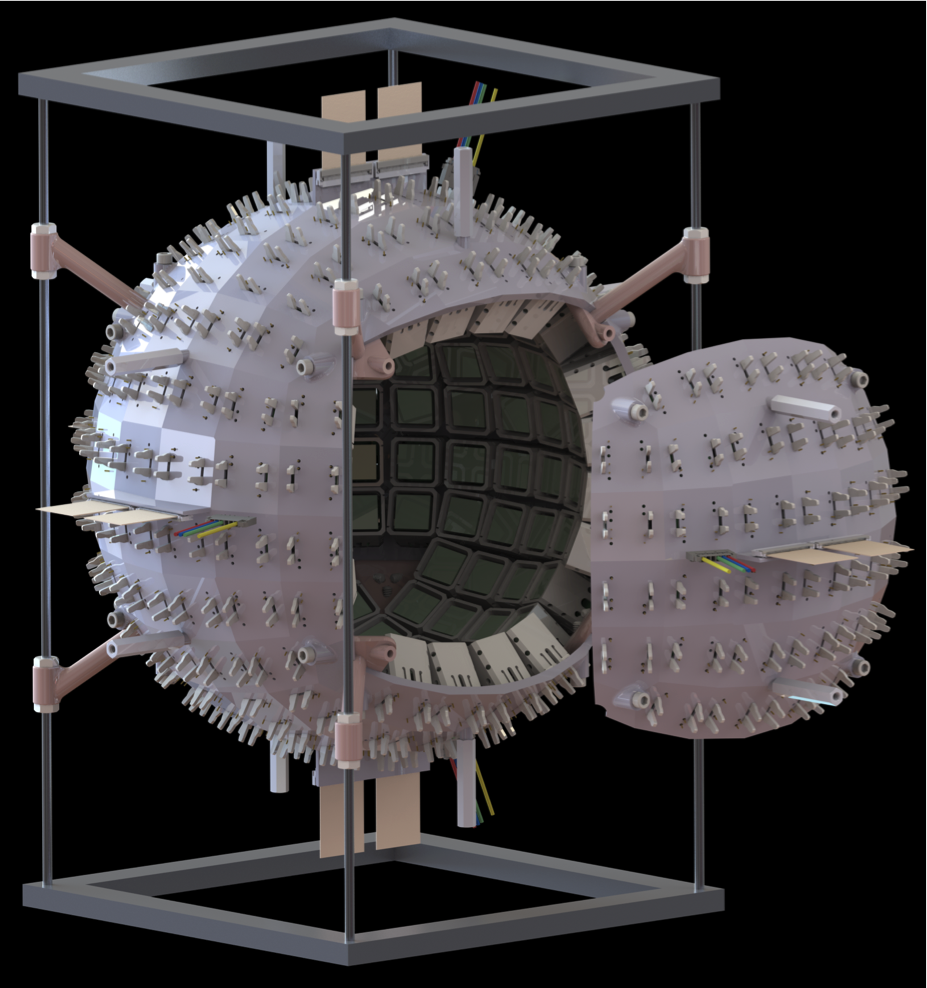
\includegraphics[height=130pt]{Figures/PRISM_Design.png} & 
	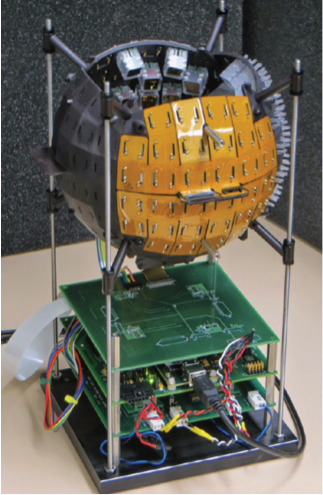
\includegraphics[height=130pt]{Figures/PRISM_Prototype.png} & 
	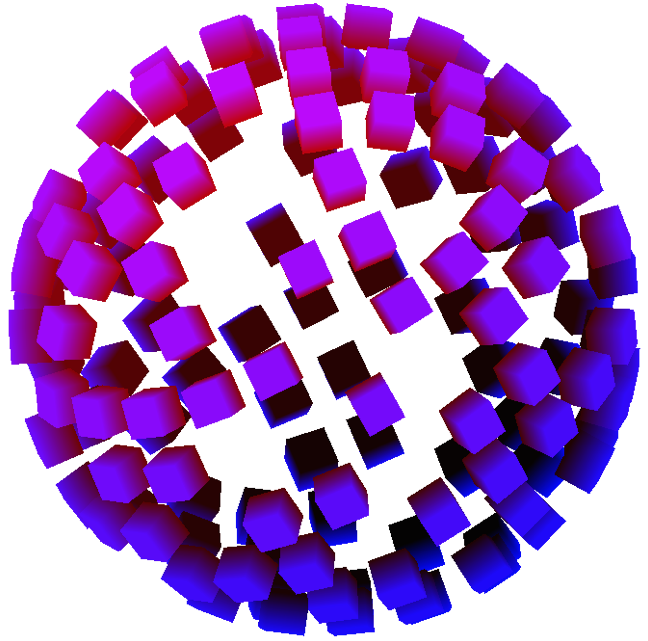
\includegraphics[height=130pt]{Figures/Masked_Configuration.png} \\
	\scriptsize{(a)} & \scriptsize{(b)} & \scriptsize{(c)} \\[-6pt]
\end{tabular}
\caption{(a) Modular design of PRISM. (b) PRISM prototype system currently under development at LBNL. (c) Example coded arrangement of detectors.}
\end{figure}






% -----------------------------------------------------------------------
\section{Mathematics}

%A simple handheld radiation detector (such as a simple NaI scintillation crystal attached to a photomultiplier tube) can be used to map radiation. The count rate is recorded while the system is moved through space, and an intensity map can be produced in 3D. This method, however, is not optimal because of the low efficiency (only one detector), the poor spatial resolution, and the dependence on the users path and proximity to the source. To produce a freely moving handheld system with high efficiency and high energy/spatial resolution, a move clever approach is needed.

\subsection{Coded Aperture Imaging}

Coded aperture is a technique first developed for X-ray astronomy and uses the principle of unique photon modulation for image reconstruction \cite{Dicke1968}. Typically an array of position sensitive photon detectors are placed behind a coded array (also referred to as an \emph{aperture} or \emph{mask}) of photon absorbing material (such as lead or tungsten). The concept is similar to a pinhole camera, however, several pinholes are used in the aperture (typically with an \emph{open fraction} of 50\% \cite{FenimoreCannon1978}) to increase the signal-to-noise-ratio (SNR) - which is necessary when attempting to image weak sources. The aperture arrays are designed such that the detected images (or \emph{shadowgrams}) uniquely correspond to a location in the image space. Reconstruction algorithms are used to decode the detected image, typically using either correlation or iterative methods \cite{FenimoreCannon1978, LangeCarson1984}.

% As each transparent element in the coded aperture acts as a pinhole, the detected image will be overlapping replicas of the source object. With the use of a reconstruction algorithm, the coded image can be decoded to result in a single image.

In the case of PRISM, there is no lead or tungsten to avoid weight and instead more detectors are used. At low energies, the CZT easily attenuates the photons and acts as a highly absorbing mask (the counts in the mask detectors can also be rejected). Moreover, using detectors instead of a passive mask increases the detection efficiency and improving weak source detection (or decreasing the \emph{minimum detectable activity} (MDA)).

As in a vast variety of physical processes, the imaging system can be described by a convolution. In order to avoid working with reflected images, as is the case when using a pinhole camera, it is typical to instead describe the system as a correlation. The imaging equation can written as
%
%To reconstruct the image, the absorbing array (typically referred to as the \emph{mask} or the \emph{aperture}) is used to deconvolve the detected image (which by itself will not reveal anything about the source location). Typically this is represented by the following:
%
\begin{equation}
	P = A \star O + N\,,
\end{equation}

\noindent where $P$ is the detected image, $A$ is the aperture, $O$ is the source object, $N$ is noise, and $\star$ is the correlation operator. In one dimension this is given by
%
\begin{equation}
	f(x) \star g(x) = \int_{-\infty}^\infty du\,g^\ast(u-x)f(u)\,.
\end{equation}

\noindent This is related to the convolution operation ($\ast$) by the adjoint operator (all functions will be real in this case, so this is simply a reflection operation)
%
\begin{equation}
	f(x) \ast g(x) = \int_{-\infty}^\infty du\,g(x-u)f(u)\,.
\end{equation}

\noindent To analytically solve for the source object $O$, the convolution theorem
%
\begin{equation}
	\mathfrak{F}(f(x) \ast g(x)) = \mathfrak{F}(f(x)) \mathfrak{F}(g(x)) = F(k)G(k)\,,
\end{equation}

\noindent is used, where $\mathfrak{F}$ is the Fourier transform operator and $k$ is spatial frequency. Applying this to Eq.(1) ultimately results in 
%
\begin{align}
	%\mathfrak{F}(P) = \mathfrak{F}(A) \mathfrak{F}(O) + \mathfrak{F}(N)\,, \\
	%\mathfrak{F}(O) = \frac{\mathfrak{F}(P)}{\mathfrak{F}(A)} + \frac{\mathfrak{F}(N)}{\mathfrak{F}(A)}\,,  \\
	%\hat{O} = \mathfrak{F}^{-1}\left(\frac{\mathfrak{F}(P)}{\mathfrak{F}(A)} + \frac{\mathfrak{F}(N)}{\mathfrak{F}(A)}\right)\,, \\
	\hat{O} = O + R\mathfrak{F}^{-1}\left( \frac{\mathfrak{F}(N)}{\mathfrak{F}(A)}\right)\,,
\end{align}

\noindent where $R$ is the reflection operator and $\mathfrak{F}^{-1}$ is the inverse Fourier Transform. This method of \emph{deconvolution} is simple and straightforward. However, since the aperture is an array of ones and zeros, the $\mathfrak{F}(A)$ term can be small, leading to large noise gain in the image. A variety of different reconstruction techniques exist, including simple (and filtered) back-projection, cross-correlation, and maximum likelihood expectation maximization (MLEM) \cite{LangeCarson1984}. Back-projection simply adds intensity to each image pixel proportional to the probability that the event originating from that pixel. However, since a single event is not unique to a single image pixel, the resulting images can be quite blurry. Cross-correlation typically uses the mask pattern to define a post-processing array, $G$, such that $A\star G$ approximates a delta function. $G$ is applied to Eq. (1) and the equation is inverted to solve for $O$. However, $A\star G$ is never a true delta function and thus the images will contain some blur. Moreover, with the spherical array in PRISM, it is unclear how $G$ would be defined. For these reasons, this report will focus solely on MLEM.

The derivation of the MLEM method is as follows. Assume the measured detector counts are Poisson distributed, such that the probability of observing a count $k$ in detector $\lambda$ is 
%
\begin{equation}
	P(z=k)  = \frac{e^{-\lambda} \lambda^k}{k!}\,,
\end{equation}

\noindent and thus the likelihood over all detector bins and image pixels is 
%
\begin{equation}
	L(X,\lambda) = \prod_{i,j\in I_i} \ \frac{e^{-C_{ij}\lambda_j} (C_{ij}\lambda_j)^{X_{ij}}}{X_{ij}!}\,,
\end{equation}

\noindent where $i$ is the detector index, $j$ is the image pixel index, $I_i$ are the set of image pixels that contribute to detector $i$, $C_{ij}$ is the probability of getting a count in detector $i$ from source $j$, or \emph{system response} (determined from simulation), $\lambda_j$ is the intensity at image pixel $j$, and $X_{ij}$ is the number of photons emitted from source $j$ to detector $i$. Also note that the total number of counts in detector $i$ is given by $Y_i=\sum_{j \in I_i} X_{ij}$. To make Eq. (6) more manageable, the log-likelihood function is typically used. The conditional expectation of the log-likelihood is taken with respect to $Y$ and the current source distribution $\lambda^n$
%
%\begin{equation}
%	\log L(X,\lambda) = \sum_i \sum_{j \in I_i} \left[ -C_{ij} \lambda_j + X_{ij} \log (C_{ij} \lambda_j) - \log (X_{ij}!) \right]\,.
%\end{equation}
%
\begin{equation}
	E[\log L(X,\lambda) | Y,\lambda^n] = \sum_i \sum_{j \in I_i} \left[   -C_{ij} \lambda_j + \frac{C_{ij}\lambda_j^n Y_i}{\sum_{k \in I_i}C_{ij}\lambda_k^n }   \log (C_{ij} \lambda_j)   \right]\,.
\end{equation}

\noindent The expectation is then maximized, by taking a partial derivative with respect to $\lambda_j$ and setting it equal to 0
 %
 \begin{equation}
	\frac{\partial}{\partial \lambda_j} E[\log L(X,\lambda) | Y,\lambda^n] = 0\,.
\end{equation}

\noindent Solving the above, the final result is concise and gives a relation between the current source distribution and the next iteration
%
 \begin{equation}
	\lambda_j^{n+1} = \frac{\lambda_j^n}{\sum\limits_{i \in J_j}C_{ij}} \sum_{i \in J_j} \frac{C_{ij}Y_i}{\sum\limits_{k \in I_i}C_{ik}\lambda_k^n}\,,
\end{equation}

\noindent where $J_j$ is the set of detectors to which image pixel $j$ contributes.

This method can be used to reconstruct the source distribution without the noise gain effects inherent in analytical deconvolution and without the blur of back-projection, but because of its iterative nature, comes at a cost of computational time. In most cases the technique can be easily vectorized and computed quickly; however, it can become difficult when attempting to reconstruct in a list-mode fashion (count by count) in real time. Furthermore, the convergence of this method is a topic of debate in the field. MLEM attempts to reduce noise and increase resolution with each iteration, however if the input data contains a significant amount of noise, there can come a point where more iterations makes the image worse. Therefore it can be difficult to define convergence criteria. In some cases, the number of iterations is fixed based on previous experience. \textcolor{red}{CITATIONS}.



% -------------------------------------------------
\subsection{Compton Imaging}

Coded aperture imaging is powerful when the photon energy is low because the modulation (or \emph{mechanical collimation}) is what produces the unique coding on the detected image. As the energy is increased, the photoelectric absorption cross-section decreases and the Compton scattering cross-section increases. The decrease in attenuation and increase in scattering will essentially remove the coded effect and blur the images. Therefore, an \emph{electric collimation} technique such as Compton imaging must be used for higher energy photons. Gamma-rays can undergo Compton scattering in a detector, depositing a detectable amount of energy, and then eventually undergo a photoelectric absorption in another detector. A variety of other scenarios exists (scatter-scatter-absorb, scatter-escape, pair produce-scatter-absorb, etc.), but this report will focus only on two-interaction tracks. By measuring the interaction positions and energy depositions of the individual interactions, the photon path can be tracked through the system. The two interactions can then be used to determine a cone of incident angles from which the incident photon originated. The image is reconstructed by the overlap of multiple cones (in 3D) or circles (in 2D).

If the incident ($E_\gamma$) and scattered gamma-ray ($E_\gamma^\prime$) energies are known, the scattering angle can be solved with the Compton scattering formula
%
\begin{equation}
\mu = \cos(\theta) = 1 + \frac{m_e c^2}{E_\gamma} - \frac{m_e c^2}{E_\gamma^\prime}\,,
\end{equation}

\noindent where $m_e c^2$ is the rest mass of the electron (= 511 keV). The positions of the scattering interaction and the subsequent photoelectric absorption define an axis. A cone of possible gamma-ray directions can then be defined and back-projected into space from the scattering interaction location. In practice, detectors have finite energy, position, and time resolution. First, finite time resolution will obscure the exact ordering of events. Coincidence gates must be defined, which will introduce random coincidences into the data. Finite position resolution will introduce uncertainty into the cone axis. Typically for a given interaction, the interaction positions are assigned to the center of the detectors. If the \emph{lever arm}, or the distance between the two interactions, is small, this effect can be large. Finally, finite energy resolution will introduce uncertainty into the calculated scattering angle and limit our ability to determine if two events came from the same initial gamma-ray. 

For a given two-interaction track, we must sequence the two events in time. First, we assume the measured energy depositions in the detectors will sum to the incident gamma-ray energy. If the $E_{tot} \leq 256$ keV, the kinematics of Eq. (11) states that the first interaction will always deposit less energy than the first. Therefore the sequence of the events can be known by comparing the energies. If $E_{tot} > 256$ keV, the sequencing will be ambiguous. Kinematic tests, such as the Compton Edge test can be used to discard forbidden sequences. The Compton Edge refers to the maximum amount of energy than can be deposited for a given Compton scattering event. It occurs when the gamma-ray undergoes a complete backscatter ($\theta = \pi$). For each sequence, we can test to see whether the first energy deposition exceeds the Compton Edge. If so, the sequence can be rejected. 

In the far-field limit (parallel rays at infinity), each cone can be projected from the origin of the image space. The image space covers all of 4$\pi$ and is defined as a unit sphere, $\mathbb{S}^2$. We define a unit vector for the cone axis as $\hat{\vec{w}}$ and a point in $\mathbb{S}^2$ as $\hat{\vec{x}}$. The dot product of these two vectors than corresponds to the cosine of the angle between them. If this angle equals the scattering angle, then the point in $\mathbb{S}^2$ is on the cone. An infinitesimally thin cone back-projected into a discretized image space would result in pixellation effects. Therefore we give the cone a small width and intensity defined by a Gaussian function. The back-projected image is then the sum of all the cones
%
\begin{equation}
b(\hat{\vec{x}}) = \sum_{i=1}^n \frac{w_i}{\sigma_i \sqrt{2\pi}} \exp\left( -\frac{(\hat{\vec{x}} \cdot \hat{\vec{w}} - \mu_i)^2}{2\sigma_i^2} \right)\,,
\end{equation}

\noindent where $i$ runs over all the cones, $\sigma$ is the width of the cone, and $w$ is the weight of the cone. The width of the cone is selected to be smaller than the expected resolution of the system, as to be able to see resolution-based effects in the image reconstruction. One may be inclined to include the uncertainty in the scattering angle from the uncertainty in the measured energies into the cone width. For a small number of cones, this will certainly help with source location, however with a large number of cones, this will simply degrade the resolution because the uncertainty is introduced twice. Imagine a large number of cones with a small width being back-projected - the uncertainty in the cones position in space will be built into its projection and over a large number of cones, will define the resolution of the system. If the uncertainty is included, the resulting image will be excessively blurred. The weight of the cones are defined in two ways. In the case of ambiguous sequences, we apply a normalized weight to each sequence proportional to the Klein-Nishina differential scattering cross-section for the two scattering angles. The sequence with a larger probability of occurring is given a larger weight. The Klein-Nishina formula is given by 
%
\begin{equation}
\frac{d\sigma}{d\Omega}(E_\gamma, \theta) = \frac{\alpha^2 r_c^2 P(E_\gamma, \theta)^2}{2} \left[ P(E_\gamma, \theta) + P(E_\gamma, \theta)^{-1} - 1 + \cos^2(\theta) \right]\,,
\end{equation}

\noindent where $\alpha$ is the fine structure constant, $r_c$ is the reduced Compton wavelength of the electron, and $P(E_\gamma, \theta)$ is given by
\begin{equation}
P(E_\gamma, \theta) = \frac{1}{1+\frac{E_\gamma}{m_e c^2}(1-\cos\theta)}\,.
\end{equation}

For all cones, we also incorporate the lever arm into the weight. Events with smaller lever arms are more likely to occur and will produce images with worse angular resolution. Therefore we apply a weight of $L^2$ where $L$ is the lever arm in order to more heavily weight the larger lever arm events \cite{Haefner2015}.


%The mathematics involved in Monte Carlo transport of photons in the detector system is quite simple. There are three main computations occurring in the simulation - sampling the distance into a material in which an interaction takes place (\emph{next collision distance}), sampling the interaction process, and, if a scattering event, sampling the energy and angle of the scattered photon. For this project, the physics of electron transport will be neglected.
%
%First, sampling the distance to interaction is done essentially by inverting the probability density function (PDF). The probability of not having an interaction (any interaction) after a distance $x$, and then having an interaction at $x$ is given by 
%%
% \begin{equation}
%	p(x) = \Sigma_t e^{-\Sigma_t x}\,, \quad x \geq 0\,,
%\end{equation}
%
%\noindent where $\Sigma_t$ is the total macroscopic cross-section of the interaction. The PDF is integrated up to a distance $x$ and set equal to a random number, $\xi \in [0,1)$
%%
% \begin{align}
%	\xi = P(x) &= \int_0^x \Sigma_t e^{-\Sigma_t s} ds \,, \\
%	&= 1-e^{-\Sigma_t x} \,.
%\end{align}
%
%\noindent Now solve for $x$ noting that $1-\xi$ is also a random number which is just replaced by $\xi$
%%
% \begin{align}
%	x = \frac{-\log(\xi)}{\Sigma_t} \,.
%\end{align}
%
%\noindent This is calculated at every step in the particle track and compared to the distance to the next boundary in the geometry. If the next collision distance is larger than the distance to the boundary, the particle is moved to the boundary and the next collision distance is resampled in the new material.
%
%Once an interaction has occurred, the type of interaction is determined by first determining the probability of each interaction occurring. If, for example, three cross-sections exist, the probability of the three occurring are given by  
%%
%\begin{align}
%	p(\sigma_1) = \frac{\sigma_1}{\sigma_1 + \sigma_2 + \sigma_3} \\
%	p(\sigma_2) = \frac{\sigma_2}{\sigma_1 + \sigma_2 + \sigma_3} \\
%	p(\sigma_3) = \frac{\sigma_3}{\sigma_1 + \sigma_2 + \sigma_3}
%\end{align}
%
%\noindent where $\sigma$ is the microscopic cross-section and $p(\sigma_1) + p(\sigma_2) + p(\sigma_3) = 1$. Using the probabilities, a random number between 0 and 1 can be generated and a section of the domain can be designated for each interaction, where the size of the domain is proportional to the probability of it occurring.
%
%Finally, if the interaction is a scattering interaction, the energy and direction of the scattered photon must be sampled. If the scattering is a Rayleigh scattering, the energy is unchanged, but the outgoing direction may be different than the incoming direction. The outgoing direction can be sampled by performing the technique above but now using the Rayleigh scattering differential cross-section as the PDF. \textbf{Show the cross-section here}. If the interaction is Compton scattering, the outgoing direction is sampled from the differential cross-section as well, also known as the Klein-Nishina formula. \textbf{Show the cross section here}. Once the outgoing direction is sampled, the outgoing energy can be calculated analytically using the Compton scattering equation. \textbf{Show the scattering equation here}. 






% -----------------------------------------------------------------------
\section{Algorithms}

The simulation is built around the Monte Carlo toolkit, Geant4. Individual particles, as well as any secondary particles produced, are tracked from birth to death given some initial conditions and underlying physics. This is accomplished by using random sampling techniques. The geometry is built first, detailing the size, position, and material of the objects in the system. Relevant physics are defined in all materials as well as for all initial and subsequently produced particles. The photoelectric effect, Compton scattering, Rayleigh scattering, and pair production were included for the gamma-rays and multiple scattering, ionization, and bremsstrahlung were included for the electrons. A particle is then given to the tracker with a particle type, energy, position, and momentum direction. Each step in the particle track is then determined by randomly sampling the next collision distance and comparing to the next boundary distance. The particle is moved accordingly and the interaction is then randomly sampled (including the interaction type, the outgoing energy and direction, and the production of any secondary particles). If any secondary particles are produced due to an interaction, the primary particle track is paused while the secondary particle tracks are followed to completion one by one. At each step (boundary crossing or interaction site) in the track, relevant information is stored in memory. This can include position, energy, direction, etc. This process continues until the particle is absorbed, leaves the system of interest, or falls below a defined threshold (e.g. $<$ 1 eV). Once the particle track is completed, the next particle is given to the tracker and the process is repeated. Following the termination of the last particle sent to the tracker, the stored information for all particles is written to disk. 

%For the system response generation, many particles are simulated for each source location. Particles are simulated at each source location sequentially. A simple overview of this algorithm is given as follows
%
%\begin{lstlisting}
%Define geometry
%Define physics
%For each source location:
%	For each incident particle:
%		Define type, energy, position, and  direction
%		While still in the system:
%			Sample next collision distance
%			Compare to next boundary distance, move accordingly
%			Sample interaction
%			Sample outgoing information and secondary particles
%			Store relevant information
%			Track any secondary particles emitted
%	Dump stored information to file 
%Exit simulation
%\end{lstlisting}

The simulation records the detector ID, event number, hit number, track ID, energy deposition, time, depth-of-interaction (distance to anode), and the interaction process for every step in the track. In practice, the system would only be able to record the detector ID, the energy deposition, the depth-of-interaction, and the time of each triggered event. 

The primary purpose of the simulation is simulate a source of gamma-rays of some energy in space. The imaging system is small, therefore most sources can be considered far-field (all rays are parallel). To implement far-field sources, a disk slightly larger than the PRISM sphere is defined on the $z$-axis. A position on the disk is randomly sampled and then rotated through space according to the location of the source. The direction of the ray is then given as the opposite of the source position in space. The result is parallel rays emanating from a disk slightly larger than the system positioned at the source location. A disk was chosen to reduce the number of photons that do not contribute to the detector response. Also implemented in the simulation are far-field ring sources and near-field point sources. The ring source uses the same implementation as the far field source, but each position is shifted randomly around a ring of some radius provided by the user. The near-field source is accomplished by randomly sampling photon directions in a cone that is slightly larger than the PRISM sphere, given a certain distance from the origin. Example visualizations are shown in Fig.~2.

\begin{figure}[htb!]
\hypertarget{fig2}{}
\centering
\begin{tabular}{ccc}
	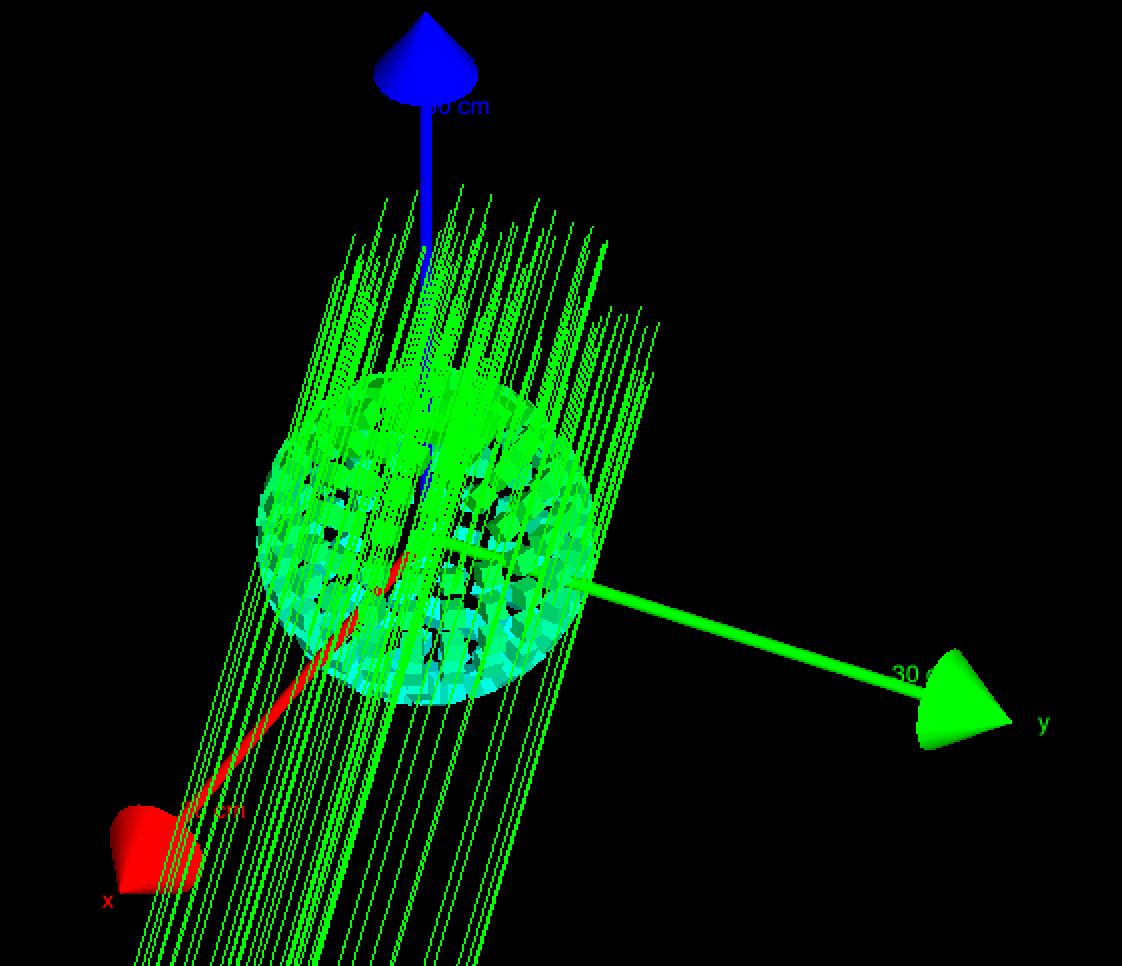
\includegraphics[height=100pt]{Figures/FarFieldVis.png} & 
	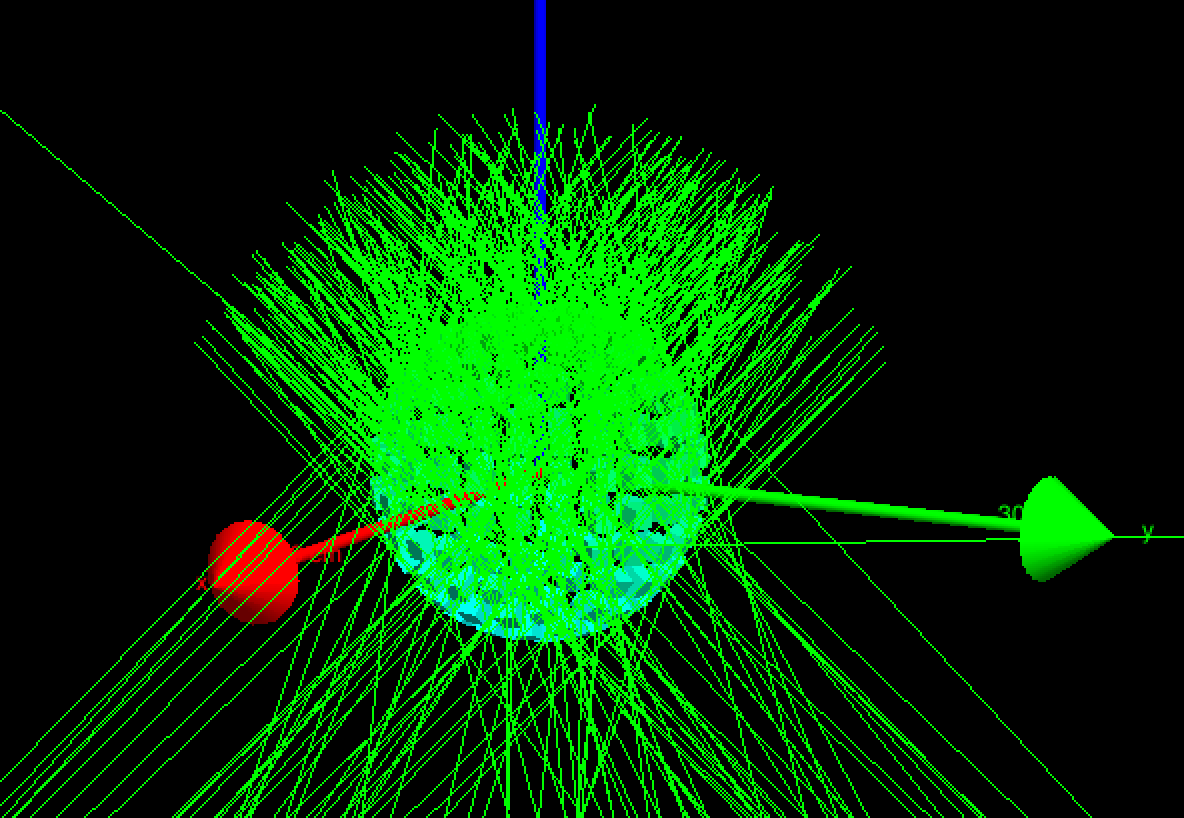
\includegraphics[height=100pt]{Figures/FarFieldRingVis.png} & 
	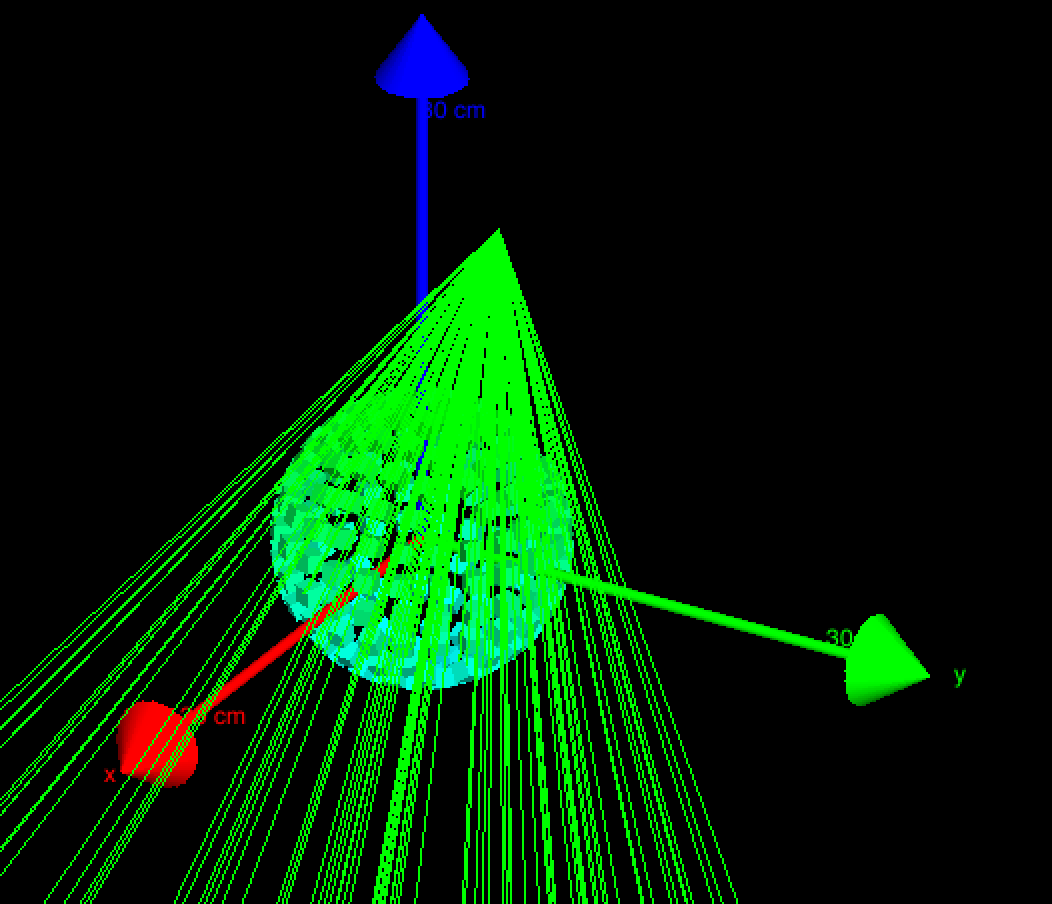
\includegraphics[height=100pt]{Figures/NearFieldVis.png} \\ [-0.5ex]
	\scriptsize{(a)} & \scriptsize{(b)} & \scriptsize{(c)}
\end{tabular}
\caption{Geant4 visualization of a (a) far-field point source, (b) far-field ring source, and (c) near-field point source}
\end{figure}


The current state of the simulation is meant to be used to either generate a full system response or produce a random data set in which image reconstruction can be done. In the case of the full system response, which is essential for coded aperture imaging, a point source is simulated at each point in the image space in order to determine the probability that a photon detected in detector $i$ came from image pixel $j$. The 4$\pi$ image space is discretized into 3072 equal area pixels on $\mathbb{S}^2$ defined using the HEALPix library \cite{Healpix2005}. For each image pixel, a user defined number of particles are simulated, and the relative responses of all the detectors are obtained. These distributions across all of the image pixels act as the coding that is used in the coded aperture reconstruction. A single source can then be simulated (potentially with a smaller number of detected events and noise included) in order to test reconstruction algorithms. The same can be said for Compton imaging, which is dependent on the number of cones to back-project. A single source can be simulated in space with some arbitrary amount of particles in order to generate a data set of sequenced events. The imaging capability can then be determine as a function of the number of cones used.

%The primary purpose of the simulation is to determine the system response, or the probability that a photon emitted from source pixel $j$ is detected in detector $i$. Therefore many particle tracks are simulated from each source pixel and the resultant response in the detectors are recorded. Currently the 4$\pi$ image space is discretized into 3072 equal area pixels defined using the HEALPix library \cite{Healpix2005} and many thousands of particles are simulated from each pixel. Therefore, the amount of data stored in each response run can be quite large and the output is in a binary file format to save space. As a part of the analysis suite, a simple binary reader in Python has been developed to extract the data into a format that can be used for image reconstruction.

In the coded aperture analysis code, only full energy absorption events are considered, so a filter is used to reject any events with less than the full energy deposited. A histogram routine is then used to bin the response in each detector for each source location. The MLEM algorithm is simple to implement in Python. Given a \emph{signal}, or an array representing the counts in each detector, an initial guess at the source distribution (\emph{image}), and the system response (\emph{response}), the vectorized algorithm can be written as follows

\begin{lstlisting}
for iteration in range(1, itr + 1):
	image = (image / numpy.sum(response, axis=0)) * numpy.dot(signal / numpy.dot(response, image), response)
\end{lstlisting}

In the Compton imaging analysis code, the output data must first be parsed for coincident events. In practice, this would be done by taking all events within some coincidence time gate following an interaction. Currently the code searches for two sequential events in different detectors that sum near a known incident energy. The coincidence events are checked agains the Compton Edge test and the accepted events are placed into a sequence array. The array is then looped over and the cone back-projection is performed, including the Klein-Nishina and lever arm weighting. Currently a cone width of 3$^\circ$ is used to avoid pixelation effects and is smaller than the expected angular resolution ($\sim10^\circ$). The back-projection intensities are added to the image array in each iteration.




%% -----------------------------------------------------------------------
%\section{Plans for Completion}
%
%The current state of the simulation is able to handle the far-field system response generation including scattering and secondary electron production, store all necessary information at each step in the particle track for coded aperture and Compton imaging, and output results to text and binary. The user is able to adjust the size of the detectors (while checking for overlaps), the coded arrangement of the detectors (using a 48 character hex code format), the indexing of the detectors and source pixels (ring or nested, see \cite{Healpix2005}), and the tracking of the electrons (on/off). More functionality will be included to allow for more geometry adjustments (radius of sphere and number of detectors), different source distributions (near field point sources and distributed sources), and varying detection scenarios (i.e.~simulate a 5 mCi \textsuperscript{133}Ba point source 10 m away for 3 minutes).
%
%The analysis suite currently has the ability to extract the simulation results from binary and generate the coded aperture system response. It can do this with and without the depth-of-interaction capability. The MLEM algorithm is also implemented and thus 4$\pi$ images can be produced using coded aperture. With the current state of the simulation, this is done in the far-field limit. Once near-field capabilities are included in the simulation, more work will need to be done in the coded aperture reconstruction algorithms to include image reconstruction in 3D. Also, a list mode (count by count) reconstruction will be implemented to simulate the capabilities of real time coded aperture imaging. Compton imaging methods still need to be implemented, including event sequencing and cone back-projection.
%
%Finally, the ultimate objective of the project is to produce a simulation and analysis framework in order to answer research questions for the novel concept of a spherical coded aperture and Compton gamma-ray imager. Simulation inputs will be developed to test the effects of finer image space discretization, different geometries (especially different coded arrangement - to determine an optimal pattern with respect coded aperture and Compton imaging performance), and different source scenarios (weak sources, distributed sources, near-field sources, short acquisition times, etc). The PRISM prototype is currently under development and is planned to be in the first stage of operation in early 2017. Physical measurements will be taken and used to validate the framework.





% -----------------------------------------------------------------------
\section{Code Use}

The Geant4 simulation is written in C\verb!++! and compiled with CMake on OSX version 10.10.5. The Geant4 version is Geant4.10.2.p1 and requires a CMake version 3.5+. This report will assume that Geant4 and CMake have been installed and sourced correctly. The \verb!compile.sh! shell script will initialize the compilation of the code. It can be run with \verb!$ sh compile.sh!. The user must input their own directory paths to the CMake executable and the Geant4 directory. A final \verb!$ make! command in the top level directory will compile the code and produce an executable called \verb!PRISM!. The code can be run by calling the executable and providing a macro file. For example: \verb!$ ./PRISM macros/run.mac!. The macro file is where the user can input various parameters for the simultion, including particle energy, source location, image pixel indexing, detector size, mask configuration (in a hexadecimal format), number of particles to run, output filename, and output file type. The \verb!run.mac! is provided as an example of the available commands and the \verb!vis.mac! macro is provided as a visualization example. Visualization in Geant4 depends heavily on the system architecture and the installed software on the machine. The visualization is not essential for this report and will not be mentioned any further. More information on each user command in the macros can be accessed during the simulation.

The system response simulation uses the macro files provided in the \verb!macros/response! directory. The set up of the simulation is done in the \verb!hp.mac! macro and the number of particles to run at each source location is specified in the \verb!main.mac! macro. To run the system response simulation, run \verb!$ ./PRISM macros/response/hp.mac!. 

Outputs will be placed in the \verb!output/! directory. The data can then be read into memory and manipulated with the Python scripts in the \verb!tools/! directory. The coded aperture system response data can be histogrammed and stored into a Python numpy array using the \verb!HistogramCodedApertureResponse.py! script by providing the output file path and energy of interest in the command line execution. The response output files can be quite large (a few gigabytes), therefore the script will perform the histogramming once and save the numpy array into a \verb!.npy! file which can be quickly read in at a later time. Currently the entire output data file is placed into memory during execution, it is the users responsibility to ensure enough RAM is available. The \verb!CodedApertureReconstruction.py! script will read in the system reponse numpy array and will perform the MLEM reconstruction on either a user defined row of the system response (to test reconstruction) or a provided output data file. The script requires the Python HEALPix package, \verb!healpy! (https://healpy.readthedocs.io/en/latest/).

The \verb!ComptonReconstruction.py! script will read in the binary simulation output data and perform the coincidence selecting, event sequencing, and cone back-projection for Compton imaging. Again, this script requires the \verb!healpy! package.



% -----------------------------------------------------------------------
\section{Test Problems and Results}

Far-field point source system response simulations were run for 60 keV and 186 keV gamma-rays with 100,000 particles at each of the 3072 source locations. A random mask was used with hexadecimal code 21524FA478BD521AB44791322B545C979943A029753854BB. Electron tracking was turned off and all energy deposition was assumed to be at the point of interaction. The output file was parsed and the system response was generated with and without depth-of-interaction. The responses are shown in Fig.~3.

\begin{figure}[htb!]
\hypertarget{fig3}{}
\centering
\begin{tabular}{cc}
	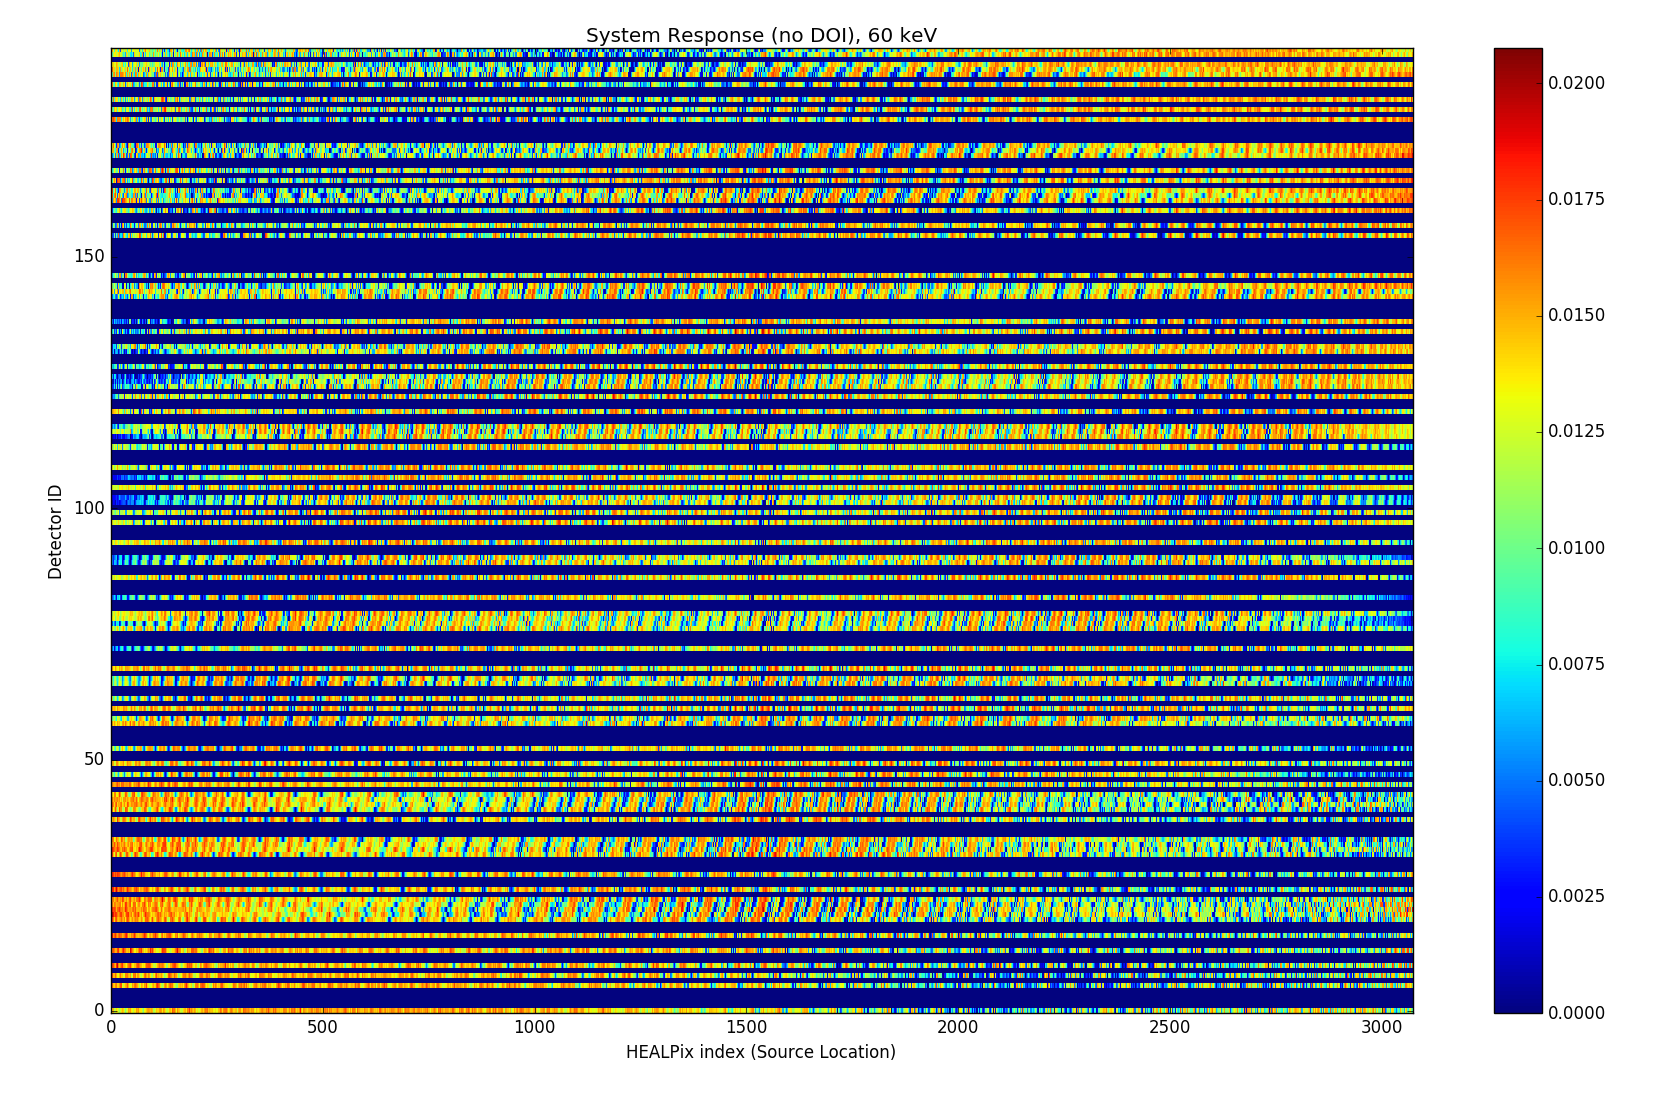
\includegraphics[height=130pt]{Figures/SystemResponse_60_noDOI.png} & 
	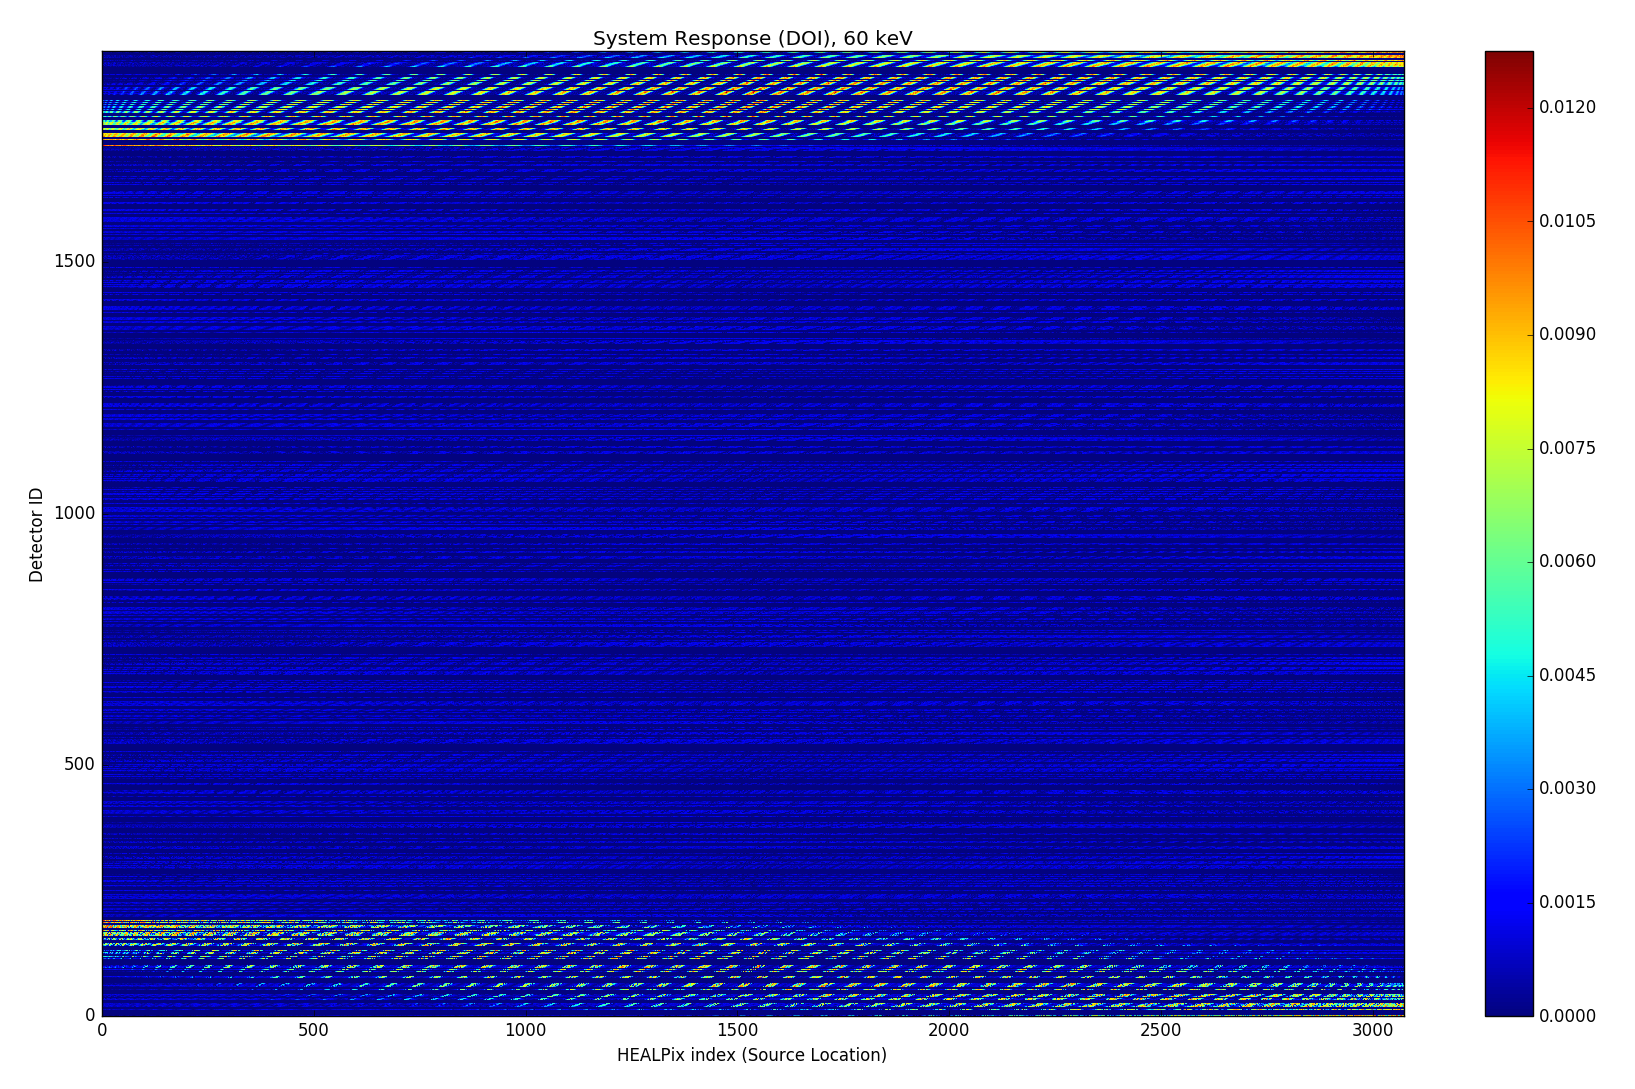
\includegraphics[height=130pt]{Figures/SystemResponse_60_DOI.png} \\ [-0.5ex]
	\scriptsize{(a)} & \scriptsize{(b)} \\ [1ex]
	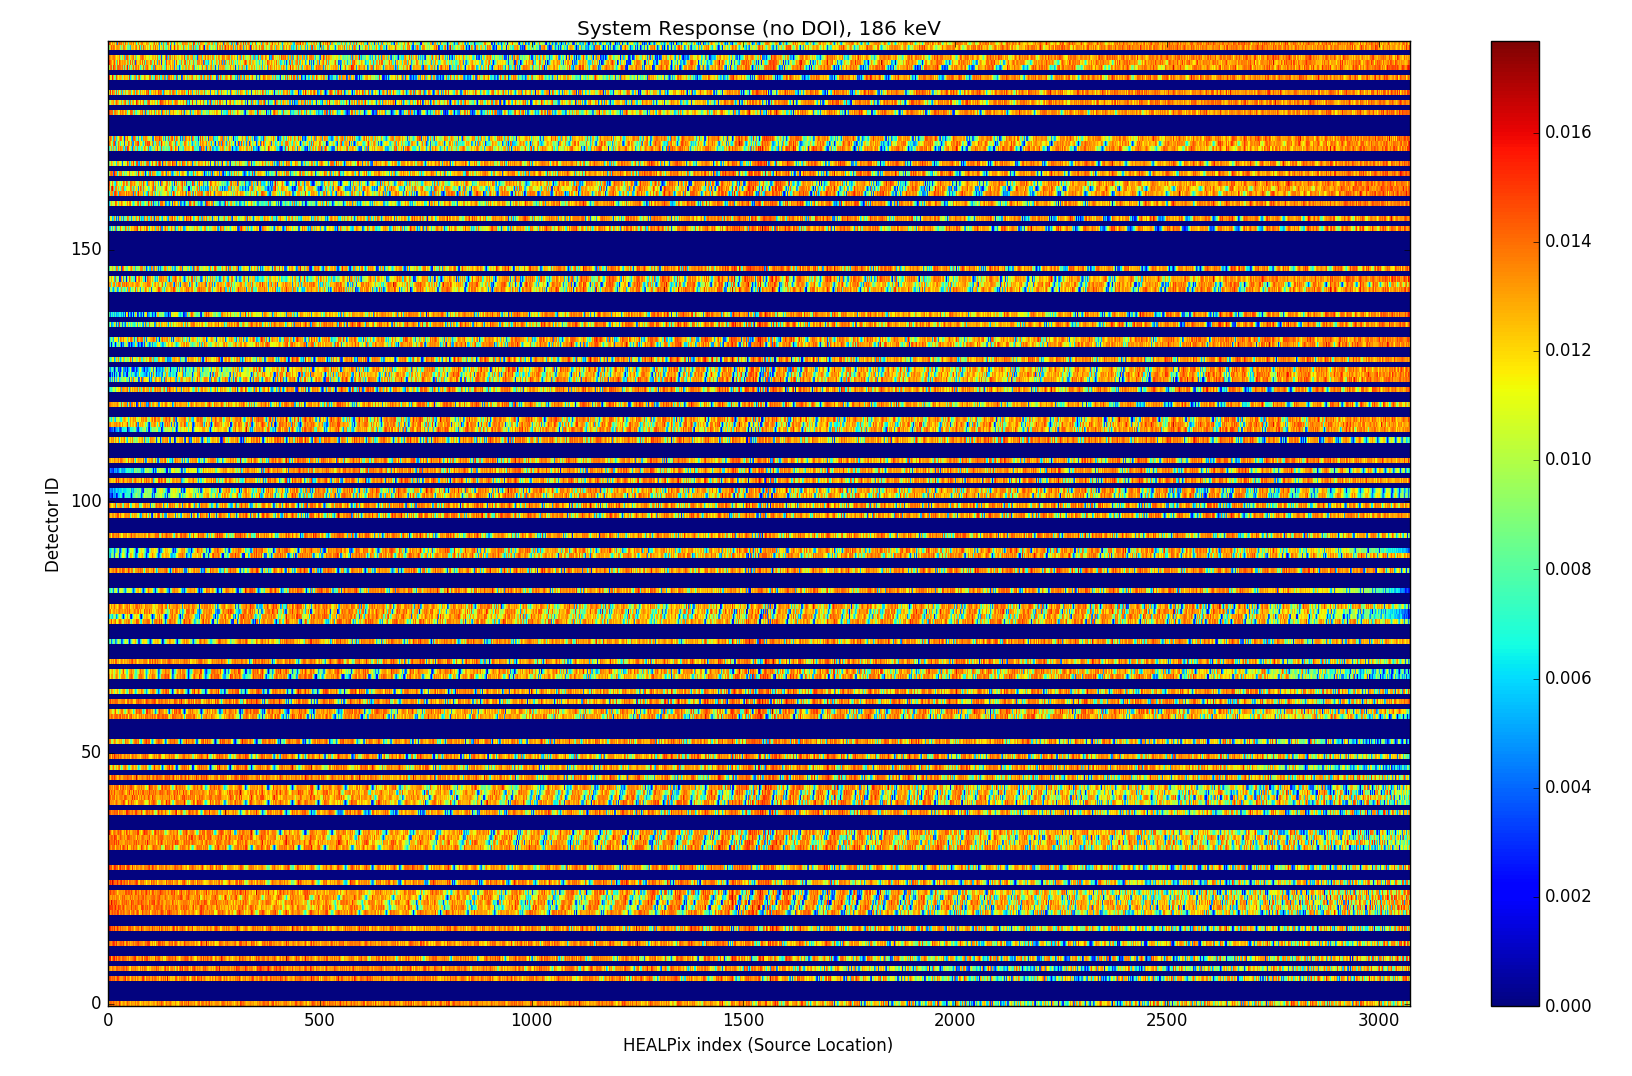
\includegraphics[height=130pt]{Figures/SystemResponse_186_noDOI.png} & 
	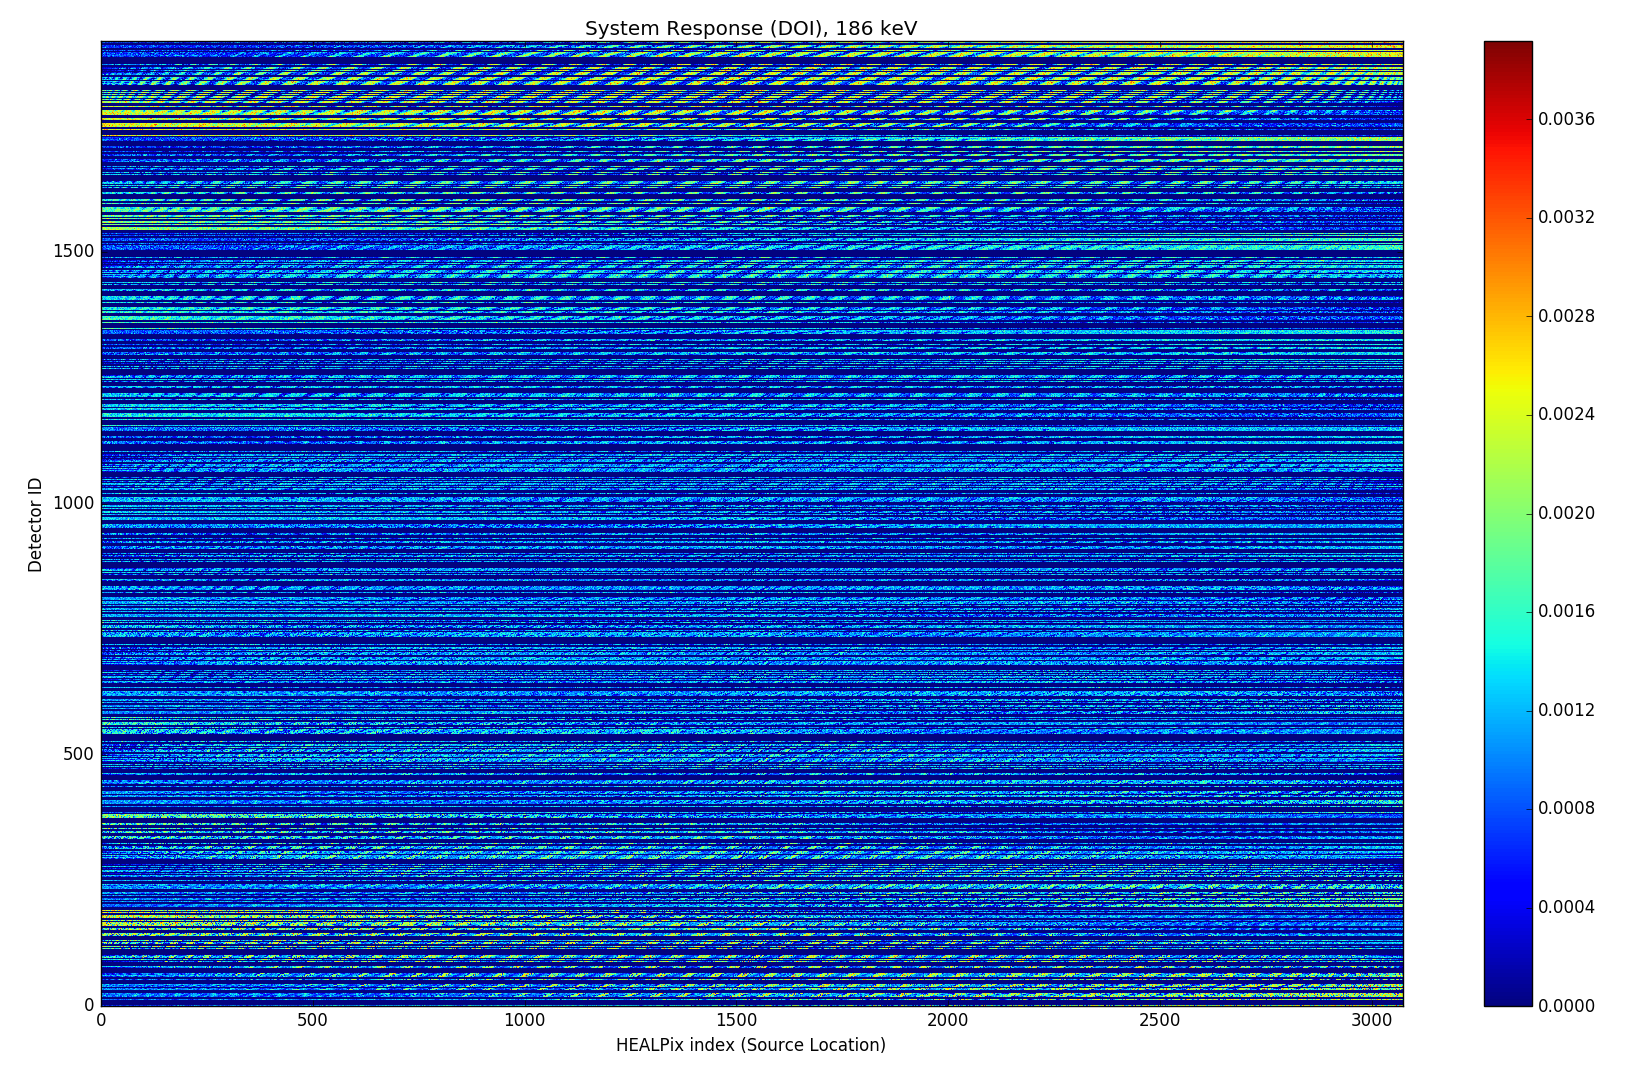
\includegraphics[height=130pt]{Figures/SystemResponse_186_DOI.png} \\ [-0.5ex]
	\scriptsize{(c)} & \scriptsize{(d)} \\[-5pt]
\end{tabular}
\caption{System response of a randomly populated mask to 60 keV gamma-rays (a) without depth-of-interaction and (b) with depth-of-interaction. System response of a randomly populated mask to 186 keV gamma-rays (a) without depth-of-interaction and (b) with depth-of-interaction.}
\end{figure}

The detectors and image pixels are indexed from the north pole to the south pole in a spiraling fashion. In each plot, the detectors are indexed to 192, however because this is a coded arrangement, some detector are missing (empty rows). It is clear that the detectors closest to the source see the largest proportion of the flux, as expected. When depth-of-interaction is included with 10 depth bins, the number of detectors is increased by a factor of 10. In this case, detectors 1 through 192 correspond to the inner bins (closest to the origin) and detectors 1728 to 1920 correspond to the bins furthest from the origin. In the 60 keV case, the gamma-ray attenuation is quite large (mean free path is a fraction of a millimeter). Most of the intensity is seen on the outer bins because they are in clear view of the source. Significant intensity is seen in the inner bins as well, accounting for the gamma-rays that pass through the open spaces of the mask and interact. The middle bins see the least amount of flux because of the large occlusion from the other detectors and the small surface area they present to the source. The large modulation of gamma-rays facilities a higher level of coding, and thus the image reconstruction should be better when depth-of-interaction is included. When the energy is increased, the depth-of-interaction behavior drastically changes as the gamma-rays can now penetrate the detectors. Therefore the intensity is distributed more throughout all the detector bins.

An arbitrary column of the system response was taken as the signal and run through the MLEM image reconstruction. The results for 60 keV with and without depth-of-interaction are shown in Fig.~4. In the depth-of-interaction case, only the inner detector responses were used as they present a compromise between the best encoding and counts. The images using 10 and 30 MLEM iterations are also shown. The true source location is shown with a blue ``X".

\begin{figure}[htb!]
\hypertarget{fig4}{}
\centering
\begin{tabular}{cc}
	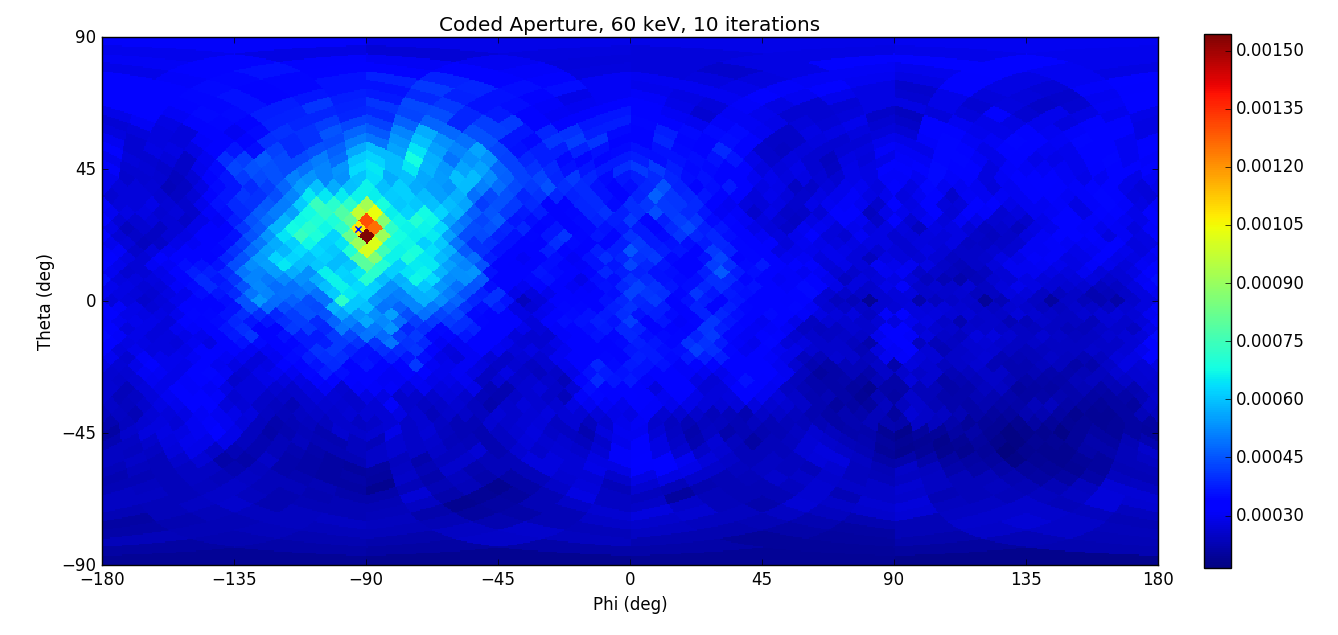
\includegraphics[height=100pt]{Figures/MLEM_60_noDOI_HP912_10itr.png} & 
	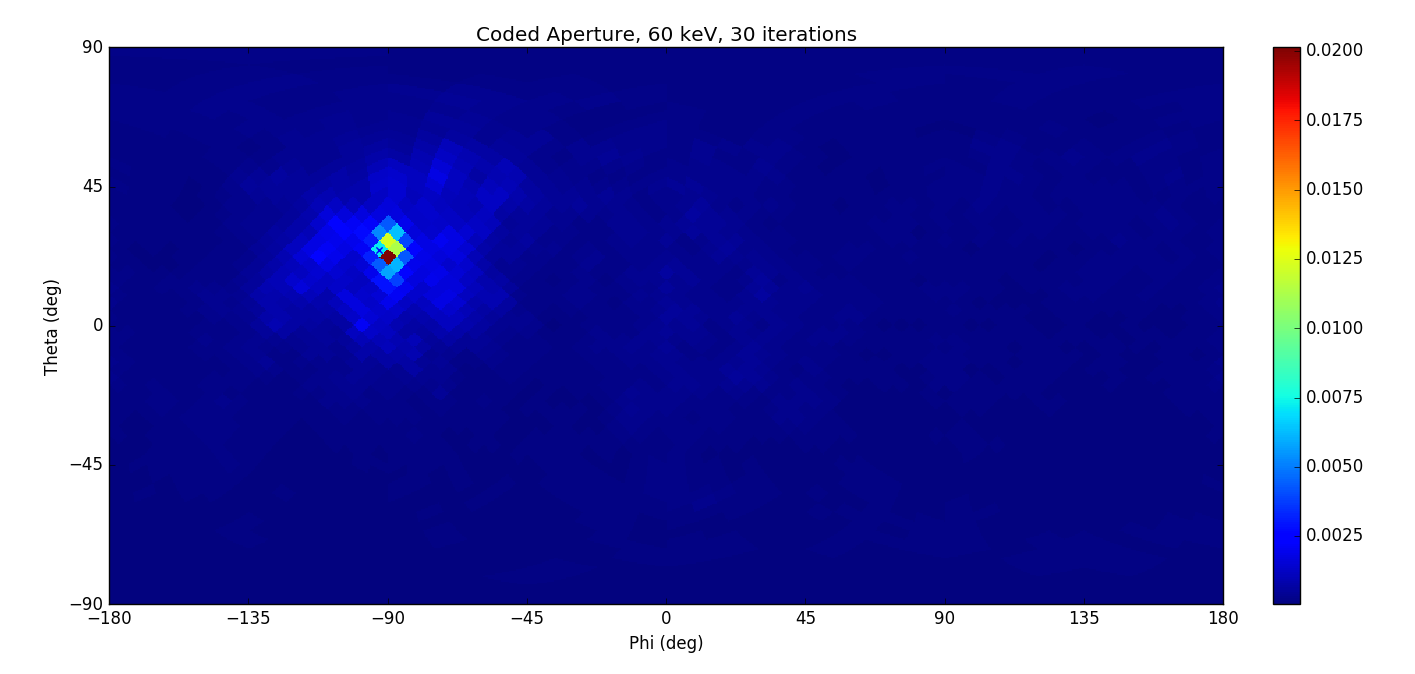
\includegraphics[height=100pt]{Figures/MLEM_60_noDOI_HP912_30itr.png} \\ [-0.5ex]
	\scriptsize{(a)} & \scriptsize{(b)} \\ [1ex]
	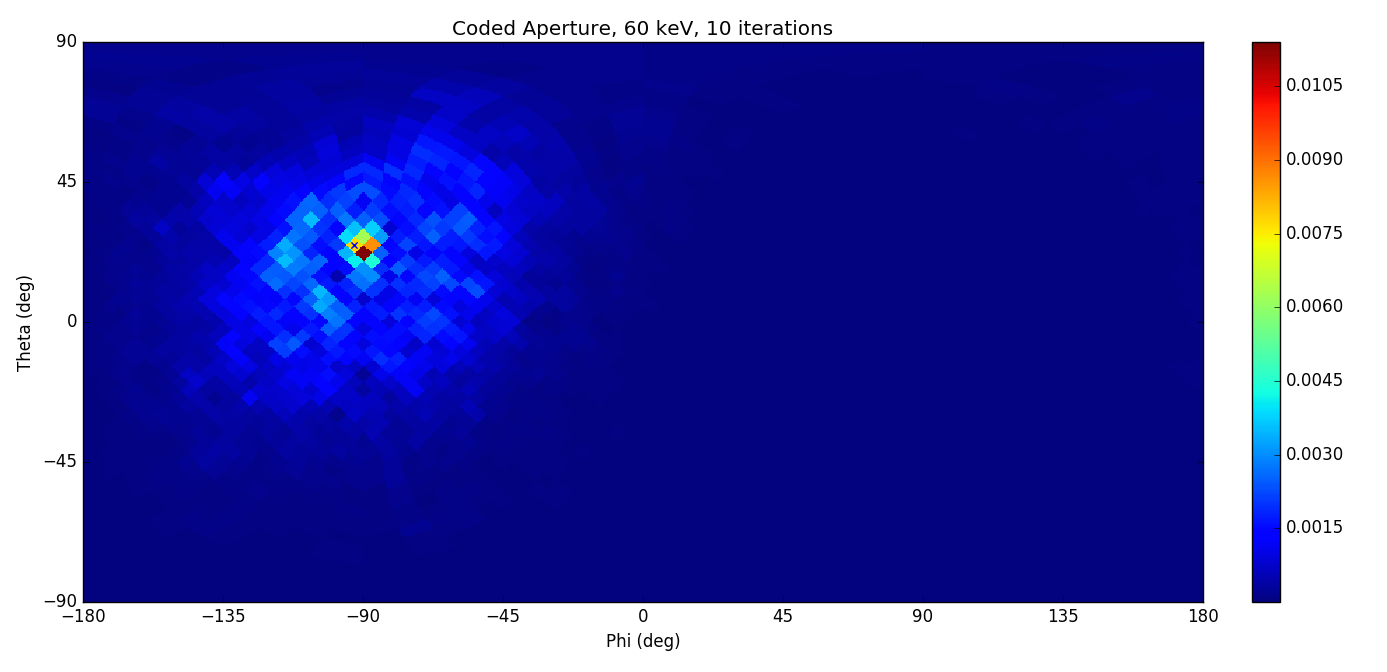
\includegraphics[height=100pt]{Figures/MLEM_60_DOI_HP912_10itr.png} & 
	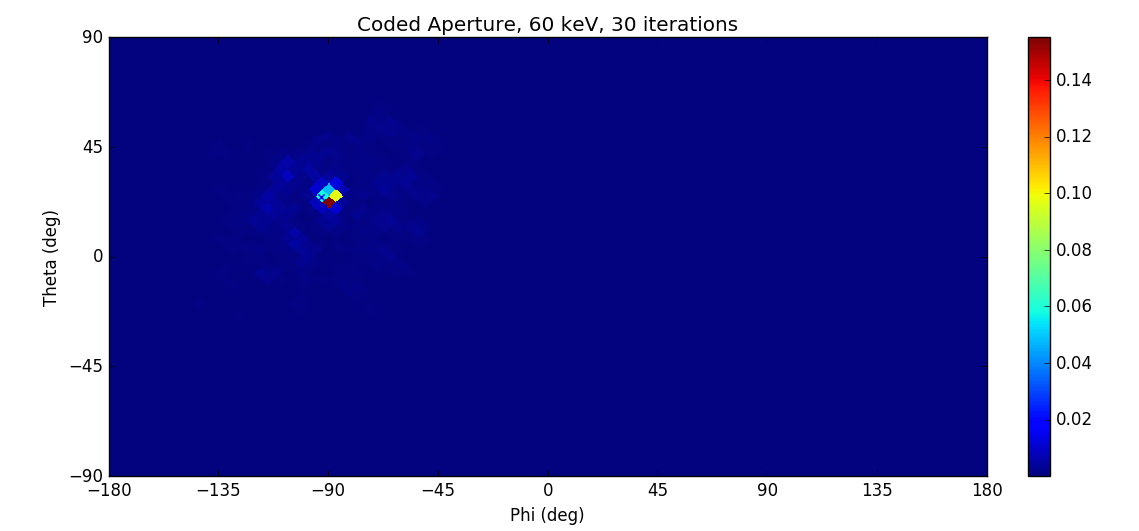
\includegraphics[height=100pt]{Figures/MLEM_60_DOI_HP912_30itr.png} \\ [-0.5ex]
	\scriptsize{(c)} & \scriptsize{(d)} \\[-5pt]
\end{tabular}
\caption{MLEM reconstruction of a 60 keV far-field point source without depth-of-interaction using (a) 10 MLEM iterations and (b) 30 MLEM iterations. MLEM reconstruction of a 60 keV far-field point source with depth-of-interaction using (a) 10 MLEM iterations and (b) 30 MLEM iterations. }
\end{figure}

As expected, the blur in the image is reduced as the number of MLEM iterations is increased. No noise was included in the simulations therefore the source location can be reconstructed exactly as the number of iterations gets larger. It is also clear that including depth-of-interaction significantly improves the image reconstruction. Each image tends to have a slight bias, however this is not surprising because an optimized mask pattern was not used. 

To test the Compton imaging analysis, a far-field point source simulation was run with 200 keV and 662 keV gamma-rays and 500,000 particles in each case. The mask was fully populated. Again, electron tracking was turned off and all energy deposition was assumed to be at the point of interaction. The output was parsed for coincident detections assuming the initial gamma-ray energy was known, and the events were sequenced. Accepted sequences were back-projected with respective Klein-Nishina and lever arm weighting. The reconstructed images with 50 and 2000 cones are shown in Fig.~5. 

\begin{figure}[htb!]
\hypertarget{fig5}{}
\centering
\begin{tabular}{cc}
	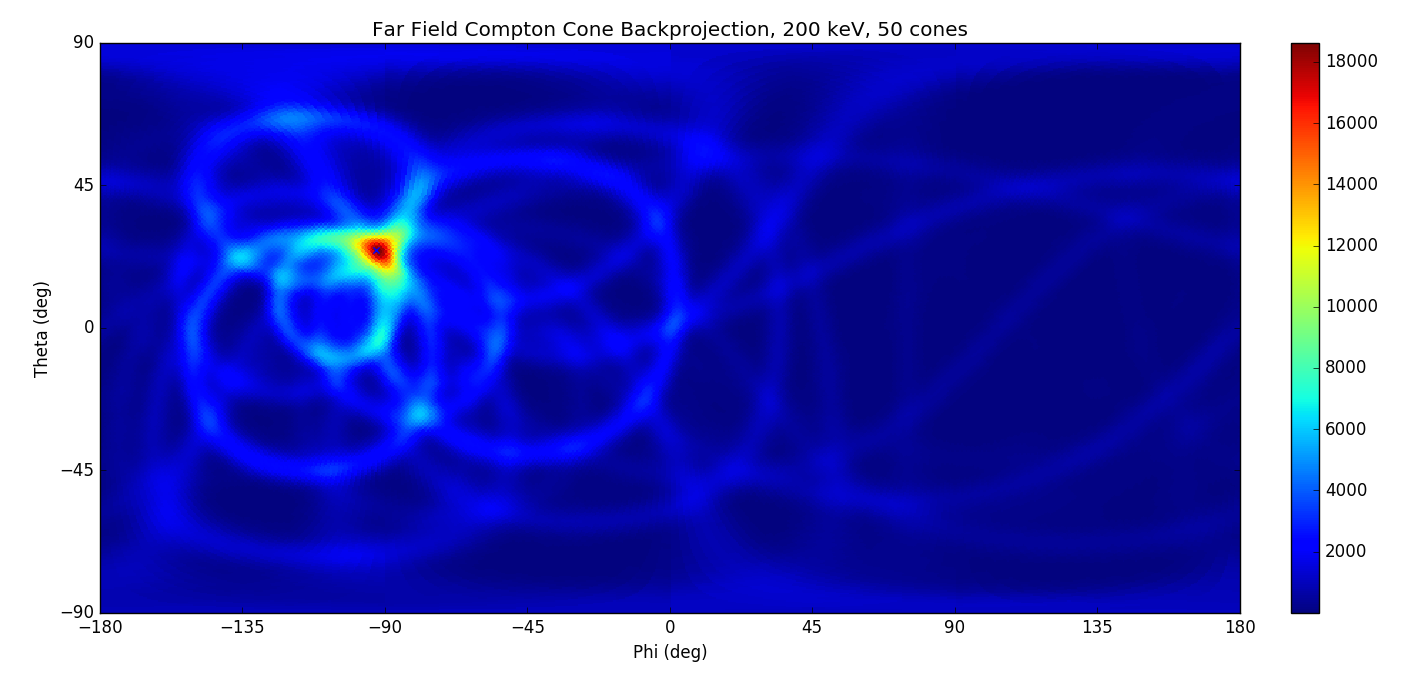
\includegraphics[height=100pt]{Figures/Compton_200_50cones.png} & 
	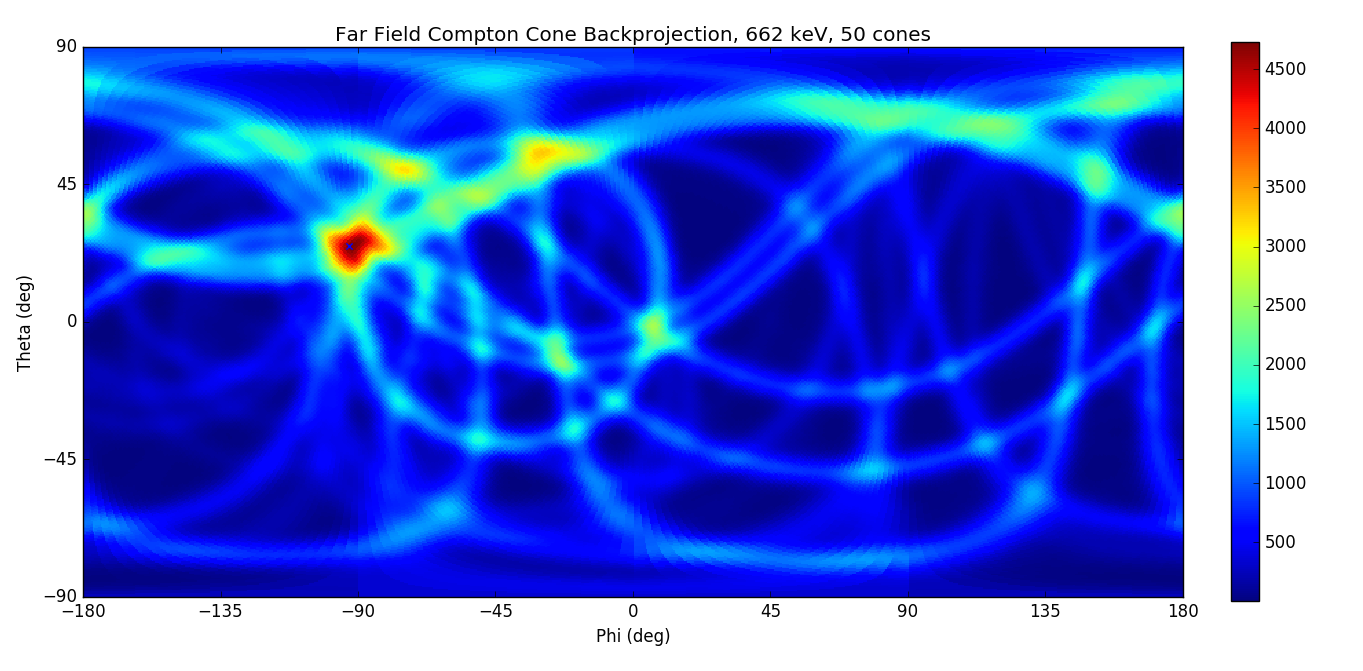
\includegraphics[height=100pt]{Figures/Compton_662_50cones.png} \\ [-0.5ex]
	\scriptsize{(a)} & \scriptsize{(b)} \\ [1ex]
	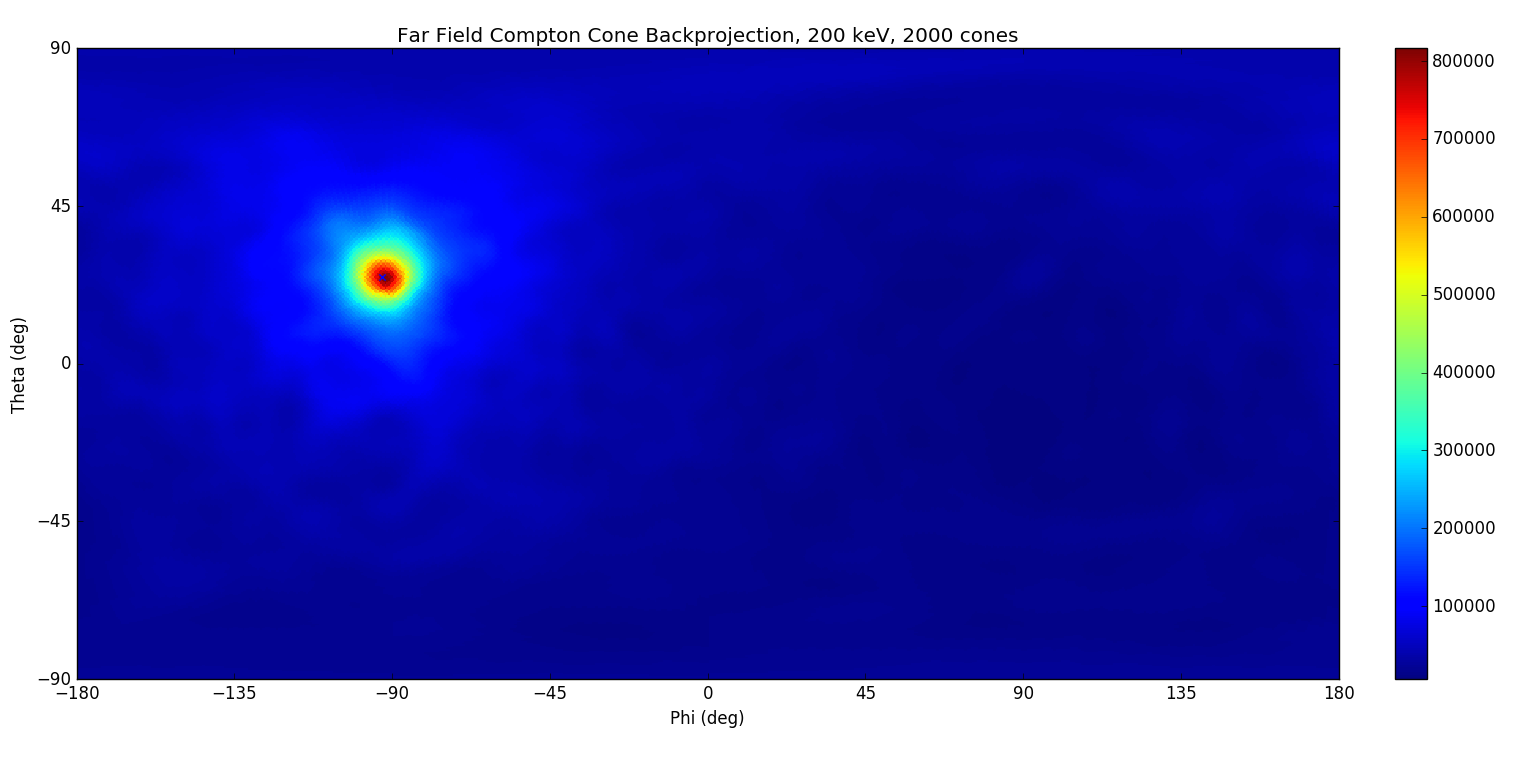
\includegraphics[height=100pt]{Figures/Compton_200_2000cones.png} & 
	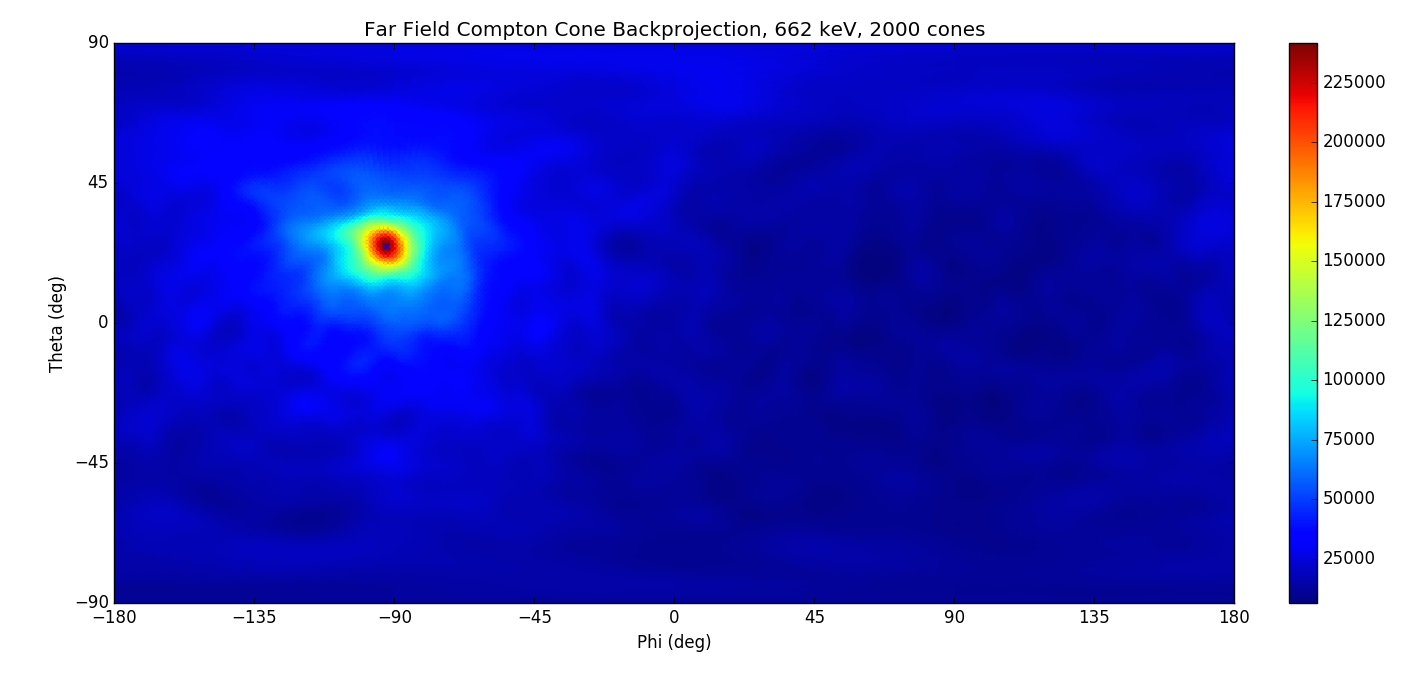
\includegraphics[height=100pt]{Figures/Compton_662_2000cones.png} \\ [-0.5ex]
	\scriptsize{(c)} & \scriptsize{(d)}
\end{tabular}
\caption{Compton cone back-projection image for a far-field (a) 200 keV and (b) 662 keV point source with 50 cones. Compton cone back-projection image for a far-field (a) 200 keV and (b) 662 keV point source with 2000 cones.}
\end{figure}

A test was also performed to verify that the first interaction always deposits less energy than the second if the incident gamma-ray energy is less than 256 keV. This is a good step towards validating the random sampling procedure that is being done internally in Geant4 for each Compton scattering interaction. The ratio of the first to second energy deposition is shown for 2000 accepted sequences for both 200 keV and 662 keV in Fig.~6. The 200 keV sequences never exceed a ratio of 1, indicating that the first interaction always deposits less energy than the first. The 662 keV sequences produce ratio both above and below 1, indicating that the amount of energy deposited first is ambiguous.

\begin{figure}[htb!]
\hypertarget{fig6}{}
\centering
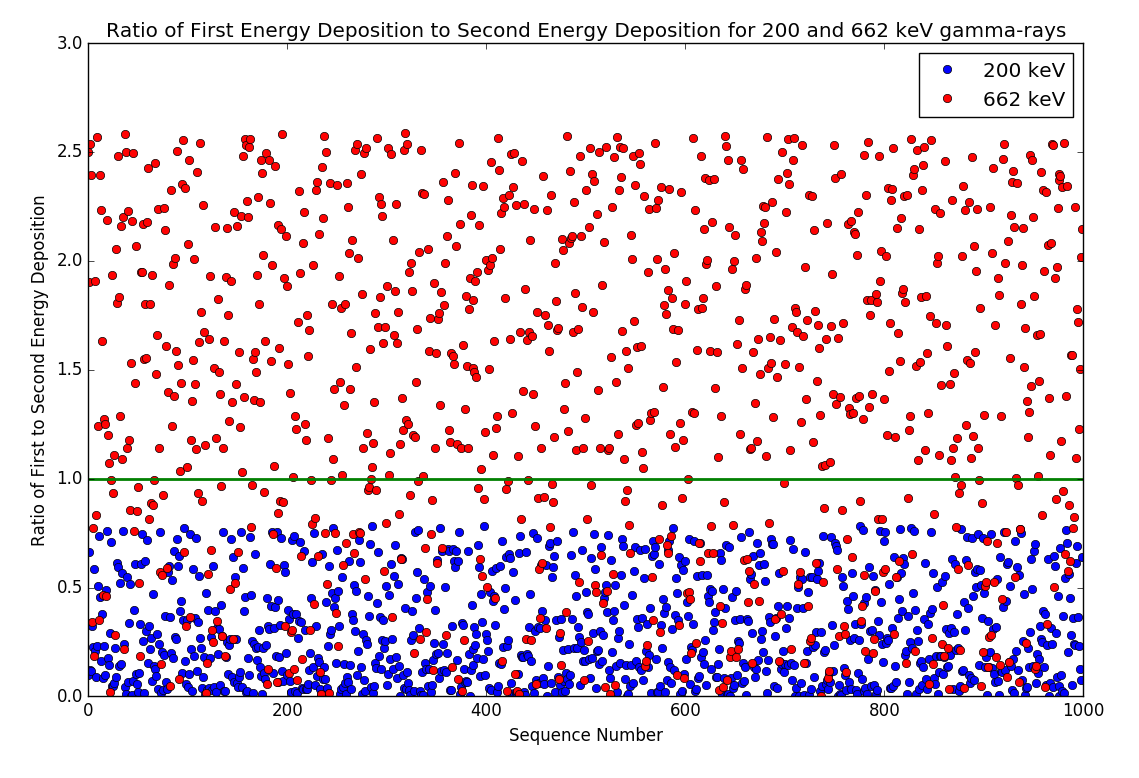
\includegraphics[height=180pt]{Figures/EnergyDepTest.png} 
\caption{Ratio of the first energy deposition to the second energy deposition for 200 keV (blue) and 662 keV (red) gamma-rays.}
\end{figure}

Finally, a far-field ring source was simulated at 60 keV (with a random mask) and 662 keV (with a fully populated mask) with 1M particles each. The image reconstructions with coded aperture and 30 iterations of MLEM (60 keV) and Compton cone back-projection (662 keV) are shown in Fig.~7. 

\begin{figure}[htb!]
\hypertarget{fig7}{}
\centering
\begin{tabular}{cc}
	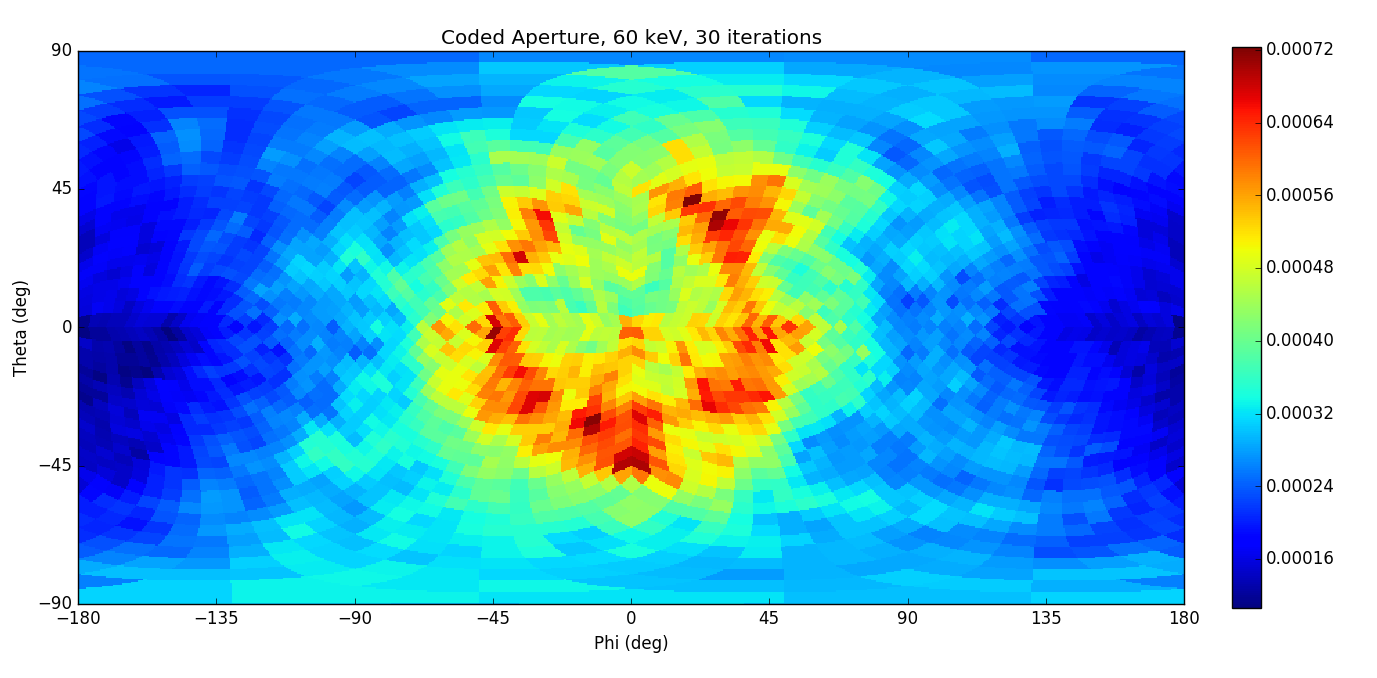
\includegraphics[height=100pt]{Figures/FarfieldRing_60.png} & 
	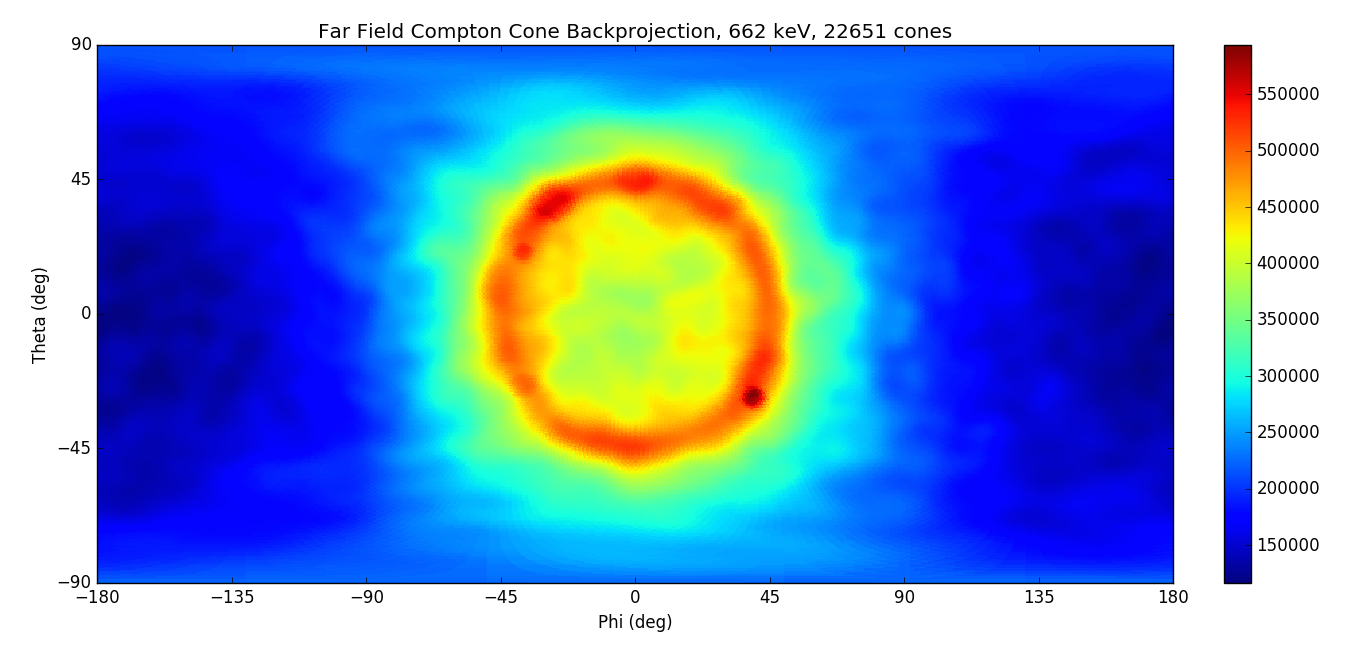
\includegraphics[height=100pt]{Figures/FarfieldRing_662.png} \\ [-0.5ex]
	\scriptsize{(a)} & \scriptsize{(b)}
\end{tabular}
\caption{(a) MLEM coded aperture image reconstruction of a far-field ring source with 60 keV gamma-rays and a random mask. (b) Compton cone back-projection image of a far field ring source with 662 keV gamma-rays and a fully populated mask.}
\end{figure}



% -----------------------------------------------------------------------
\section{Summary/Conclusions}

The PRISM imaging system is a handheld, broad energy sensitive, high efficiency gamma-ray imager currently under development at LBNL. The spherical design of PRISM is the first of its kind and will facilitate 4$\pi$ imaging in both coded aperture and Compton imaging modalities. The initial Geant4 simulation used as a ray-tracer for preliminary studies has been upgraded to include scattering, secondary electron production, depth-of-interaction readout, simple geometry modifications, and near-field and extended sources. Analysis tools were developed to parse the Geant4 output files and perform MLEM image reconstruction of coded aperture data and cone back-projection for Compton data. In both cases, the reconstruction produced reasonable images that behaved as expected for various energies, iterations, depth-of-interaction, and number of cones. The results of this project have demonstrated the 4$\pi$ imaging concept of a spherical CZT based gamma-ray imaging system and have laid the groundwork for further analysis.


\subsection{Future work}

Many studies still need to be conducted, such as multiple far-field point sources, different extended sources, and near-field sources. As the source is brought closer to the detector system, static 3D imaging may be possible with coded aperture (using magnification effects) and Compton imaging (back-projecting cones into $\mathbb{R}^3$ instead of $\mathbb{S}^2$). Moreover, since the system is handheld, the concept of including motion into the simulation must be explored. This will also include 3D tomographic imaging and real-time imaging - both quite challenging problems. PRISM will also be equipped with a LiDAR and visual camera in order to fuse contextual information with the radiation map. This will require an investigation into Simultaneous Location And Mapping (SLAM) algorithms and exploring how contextual information can be used to constrain the imaging procedure. More complex Compton reconstruction will be explored, including filtered back-projection and MLEM. The effect of including DOI in the Compton reconstruction will be studied. Event sequencing for events with greater than two interactions will be implemented, as well as appropriate energy and position blurring in the detector response and image reconstruction. Finally, geometry manipulation will be made more flexible to facilitate systematic studies of system performance as a function of detector size, sphere radius, detector spacing, mask configuration, etc. This will be critical in the future design versions of PRISM to optimize the coded aperture and Compton imaging capability for a given geometry. 




%% -----------------------------------------------------------------------
%\section{Appendix}
%\subsection{blah}
%
%...







% -----------------------------------------------------------------------
\bibliographystyle{apsrev4-1}
\bibliography{References/references}


\end{document}

